\documentclass[11pt,a4paper,openany]{book}

% -------------------------------------------------------------------------
% PACKAGES
% -------------------------------------------------------------------------
\usepackage[utf8]{inputenc}
\usepackage[T1]{fontenc}
\usepackage{lmodern}
\usepackage[margin=0.75in]{geometry}
\usepackage{microtype}
\usepackage{graphicx}
\usepackage{xcolor}
\usepackage{booktabs}
\usepackage{longtable}
\usepackage{tabularx}
\usepackage{array}
\usepackage{enumitem}
\usepackage{fancyhdr}
\usepackage{tikz}
\usetikzlibrary{arrows.meta, shapes.geometric, shapes.misc, positioning, fit, backgrounds, calc}
\usepackage[most]{tcolorbox}
\usepackage{imakeidx}
\usepackage[
    colorlinks=true,
    plainpages=false,
    pdfpagelabels=true,
    linkcolor=navyblue,
    urlcolor=tealaccent,
    citecolor=navyblue,
    pdftitle={Deployed ERP Operations Workbook \& Visual Dataflow Guide},
    pdfauthor={ERP Operations Team}
]{hyperref}

% -------------------------------------------------------------------------
% COLOR PALETTE
% -------------------------------------------------------------------------
\definecolor{navyblue}{RGB}{20, 54, 93}
\definecolor{tealaccent}{RGB}{13, 115, 119}
\definecolor{softblue}{RGB}{236, 243, 250}
\definecolor{softgreen}{RGB}{235, 247, 240}
\definecolor{softamber}{RGB}{254, 246, 230}
\definecolor{softred}{RGB}{253, 237, 236}
\definecolor{softpurple}{RGB}{244, 239, 250}
\definecolor{bordergray}{RGB}{175, 185, 195}
\definecolor{darkgray}{RGB}{55, 65, 81}
\definecolor{pinred}{RGB}{192, 57, 43}

% -------------------------------------------------------------------------
% INDEX SETUP
% -------------------------------------------------------------------------
\makeindex[columns=2, title=Alphabetical Index, intoc]

% -------------------------------------------------------------------------
% HEADERS & FOOTERS
% -------------------------------------------------------------------------
\pagestyle{fancy}
\fancyhf{}
\fancyhead[L]{\small\color{darkgray}\textbf{Deployed ERP Portal} --- Operations Workbook \& Flow Guide}
\fancyhead[R]{\small\color{darkgray}\leftmark}
\fancyfoot[L]{\small\color{darkgray}Live Production Operations (Generic Template --- Zero Real Data)}
\fancyfoot[R]{\small\color{darkgray}Page \thepage}
\renewcommand{\headrulewidth}{0.5pt}
\renewcommand{\footrulewidth}{0.4pt}

% -------------------------------------------------------------------------
% FIELD MARKER PIN & CALLOUT BOXES
% -------------------------------------------------------------------------
\newcommand{\pin}[1]{%
    \tikz[baseline=(char.base)]{%
        \node[shape=circle, fill=pinred, text=white, inner sep=1.2pt, font=\tiny\bfseries] (char) {#1};%
    }%
}

\newtcolorbox{webframe}[2]{
    colback=white,
    colframe=navyblue,
    colbacktitle=navyblue,
    coltitle=white,
    fonttitle=\footnotesize\bfseries\ttfamily,
    title={WEBSITE: https://<domain>/app/#1 \hfill [#2]},
    breakable,
    arc=3pt,
    boxrule=0.9pt,
    top=4pt, bottom=4pt, left=6pt, right=6pt
}

\newtcolorbox{rulebox}[1]{
    colback=softamber,
    colframe=orange!75!black,
    fonttitle=\small\bfseries,
    title=Business Rule: #1,
    breakable,
    arc=3pt,
    boxrule=0.8pt,
    top=3pt, bottom=3pt
}

\newtcolorbox{exercisebox}[1]{
    colback=softgreen,
    colframe=tealaccent,
    fonttitle=\small\bfseries,
    title=Practice Lab: #1,
    breakable,
    arc=3pt,
    boxrule=0.8pt,
    top=3pt, bottom=3pt
}

\newtcolorbox{cautionbox}[1]{
    colback=softred,
    colframe=red!75!black,
    fonttitle=\small\bfseries,
    title=Validation Block / Alert: #1,
    breakable,
    arc=3pt,
    boxrule=0.8pt,
    top=3pt, bottom=3pt
}

% -------------------------------------------------------------------------
% TIKZ DIAGRAM STYLES
% -------------------------------------------------------------------------
\tikzset{
    startstop/.style={
        rectangle, rounded corners=6pt, minimum width=2.8cm, minimum height=0.85cm,
        text centered, draw=navyblue, fill=navyblue, text=white, font=\footnotesize\bfseries, align=center
    },
    process/.style={
        rectangle, rounded corners=3pt, minimum width=3.0cm, minimum height=0.85cm,
        text centered, draw=navyblue, fill=softblue, text=black, font=\footnotesize, align=center
    },
    rolebox/.style={
        rectangle, rounded corners=2pt, minimum width=2.8cm, minimum height=0.8cm,
        text centered, draw=tealaccent, fill=softgreen, text=black, font=\footnotesize\bfseries, align=center
    },
    decision/.style={
        diamond, aspect=2.2, minimum width=2.3cm, minimum height=0.85cm,
        text centered, draw=orange!75!black, fill=softamber, text=black, font=\scriptsize\bfseries, align=center
    },
    docnode/.style={
        rectangle, rounded corners=3pt, minimum width=2.9cm, minimum height=0.85cm,
        text centered, draw=purple!70!black, fill=softpurple, text=black, font=\footnotesize, align=center
    },
    datanode/.style={
        rectangle, rounded corners=2pt, minimum width=2.7cm, minimum height=0.75cm,
        text centered, draw=tealaccent!85!black, fill=white, text=black, font=\scriptsize, align=center
    },
    uibox/.style={
        rectangle, rounded corners=2pt, draw=bordergray, fill=softblue!45,
        font=\scriptsize, align=left, inner sep=4pt
    },
    uibtn/.style={
        rectangle, rounded corners=2pt, draw=navyblue, fill=navyblue!12,
        font=\scriptsize\bfseries, text=navyblue, inner sep=3pt
    },
    arrow/.style={
        ->, >=Stealth, thick, draw=navyblue
    },
    dataarrow/.style={
        ->, >=Stealth, thick, draw=tealaccent
    },
    backarrow/.style={
        ->, >=Stealth, thick, dashed, draw=pinred
    }
}

% =========================================================================
% DOCUMENT START
% =========================================================================
\begin{document}

% -------------------------------------------------------------------------
% TITLE PAGE
% -------------------------------------------------------------------------
\begin{titlepage}
    \centering
    \vspace*{0.8cm}
    {\Large \color{tealaccent}\textbf{DEPLOYED ENTERPRISE RESOURCE PLANNING PORTAL}}\\[0.3cm]
    \rule{\textwidth}{1.5pt}\\[0.5cm]
    {\Huge \color{navyblue}\textbf{Visual Operations Workbook}}\\[0.25cm]
    {\Large \color{darkgray}Flowcharts, Website Field Markings \& Cross-Module Dataflow Guide}\\[0.4cm]
    \rule{\textwidth}{1.5pt}\\[0.9cm]

    \begin{tcolorbox}[colback=softblue, colframe=navyblue, width=0.95\textwidth, arc=4pt]
        \begin{tabularx}{\textwidth}{l X}
            \textbf{Scope:} & Deployed Live ERP Portal (\texttt{https://<deployed-domain>/app}) --- Daily Operations \\
            \textbf{Modules:} & Company, Users/Roles, Vendors, Equipment, PO, Proforma Invoice, Purchase Invoice, Payment Entry \\
            \textbf{Design:} & Minimal Text, Maximum Flowcharts, Generic Placeholders, Marked Website Frames \\
            \textbf{ID Patterns:} & \texttt{EQ-\#\#\#\#\#} $\cdot$ \texttt{SRIPO-\#\#\#\#} $\cdot$ \texttt{SRIPOREF-\#\#\#\#} $\cdot$ \texttt{SRI/PI/YYYY-\#\#\#\#} $\cdot$ \texttt{ACC-PINV-YYYY-\#\#\#\#\#} $\cdot$ \texttt{ACC-PAY-YYYY-\#\#\#\#\#}
        \end{tabularx}
    \end{tcolorbox}

    \vspace{0.8cm}
    \resizebox{0.92\textwidth}{!}{%
    
\begin{tikzpicture}[node distance=0.7cm and 0.8cm]
        \node (m) [rolebox] {Masters\\Company / User / Vendor / Equip};
        \node (po) [process, right=of m] {Vendor PO\\(\texttt{SRIPO-\#\#\#\#})};
        \node (app) [startstop, right=of po] {Approved PO\\(\texttt{SRIPOREF-\#\#\#\#})};
        \node (inv) [docnode, right=of app] {PI / Purchase Inv.\\(Tax \& Ledger)};
        \node (pay) [startstop, right=of inv] {Payment Entry\\(Draft $\rightarrow$ Cleared)};
        \draw [arrow] (m) -- (po);
        \draw [arrow] (po) -- (app);
        \draw [arrow] (app) -- (inv);
        \draw [arrow] (inv) -- (pay);
    \end{tikzpicture}}

    \vfill
    \begin{tabular}{ll}
        \toprule
        \textbf{Edition} & 3.0 --- Deployed Visual Flow \& Field-Mapping Manual \\
        \textbf{Data Policy} & 100\% Generic Placeholders (\texttt{<Company>}, \texttt{<Tax ID>}, \texttt{<Vendor>}, \texttt{<Amount>}) \\
        \textbf{Prerequisites} & Active Browser Login to Deployed Portal (No Installation Required) \\
        \bottomrule
    \end{tabular}
    \vspace*{0.6cm}
\end{titlepage}

% -------------------------------------------------------------------------
% FRONT MATTER
% -------------------------------------------------------------------------
\frontmatter
\tableofcontents
\clearpage
\listoffigures
\listoftables
\clearpage

% -------------------------------------------------------------------------
% PREFACE
% -------------------------------------------------------------------------
\chapter*{Preface: Visual Guide Conventions}
\addcontentsline{toc}{chapter}{Preface: Visual Guide Conventions}
\index{User Guide!Conventions}

\begin{itemize}[leftmargin=1.5em, itemsep=3pt]
    \item \textbf{Deployed System Assumption:} All steps operate directly inside the live browser portal at \texttt{https://<deployed-domain>/app}.
    \item \textbf{Screenshot Reference Frames:} Each chapter provides a marked UI layout frame representing the \textbf{Actual Deployed Website Form}, with numbered red pins \pin{X1} indicating where live website screenshots and operator inputs align.
    \item \textbf{Dataflow Arrows:} Teal arrows (\tikz[baseline=-0.5ex]\draw[dataarrow](0,0)--(0.6,0);) show automatic field inheritance between records; navy arrows show workflow actions; dashed red arrows show rejection loops.
    \item \textbf{Generic Placeholders:} All tax numbers, bank accounts, entities, vendors, and values use generic tokens (\texttt{<Tax Registration ID>}, \texttt{<Vendor Name>}, \texttt{<Amount>}).
\end{itemize}

\begin{figure}[htbp]
    \centering
    \resizebox{\textwidth}{!}{%
    \begin{tikzpicture}[node distance=0.8cm and 1.0cm]
        \node (s1) [rolebox] {1. Company Setup\\(\pin{C1}--\pin{C8})};
        \node (s2) [rolebox, right=of s1] {2. Users \& Roles\\(\pin{U1}--\pin{U5})};
        \node (s3) [rolebox, right=of s2] {3. Vendor \& Equip.\\(\pin{V1}--\pin{V8}, \pin{E1}--\pin{E6})};
        \node (s4) [process, right=of s3] {4. Vendor PO\\(\pin{PO1}--\pin{PO12})};
        \node (s5) [docnode, right=of s4] {5--6. PI / Bill\\(\pin{PI*}, \pin{INV*})};
        \node (s6) [startstop, right=of s5] {7. Payment Entry\\(\pin{PE1}--\pin{PE10})};
        \draw [arrow] (s1) -- (s2);
        \draw [arrow] (s2) -- (s3);
        \draw [arrow] (s3) -- (s4);
        \draw [arrow] (s4) -- (s5);
        \draw [arrow] (s5) -- (s6);
    \end{tikzpicture}}
    \caption{Manual Roadmap: Chapter Sequence and Field Pin Prefixes}
    \label{fig:manual-roadmap}
\end{figure}

% =========================================================================
% MAIN MATTER
% =========================================================================
\mainmatter

% -------------------------------------------------------------------------
% CHAPTER 1: MASTER FLOW & ARCHITECTURE
% -------------------------------------------------------------------------
\chapter{End-to-End Workflow \& Cross-Module Dataflow}
\index{Workflow!End-to-End Overview}\index{Dataflow!Master Architecture}

\section{Master Procurement-to-Payment Flowchart}

\begin{figure}[htbp]
    \centering
    \resizebox{\textwidth}{!}{%
    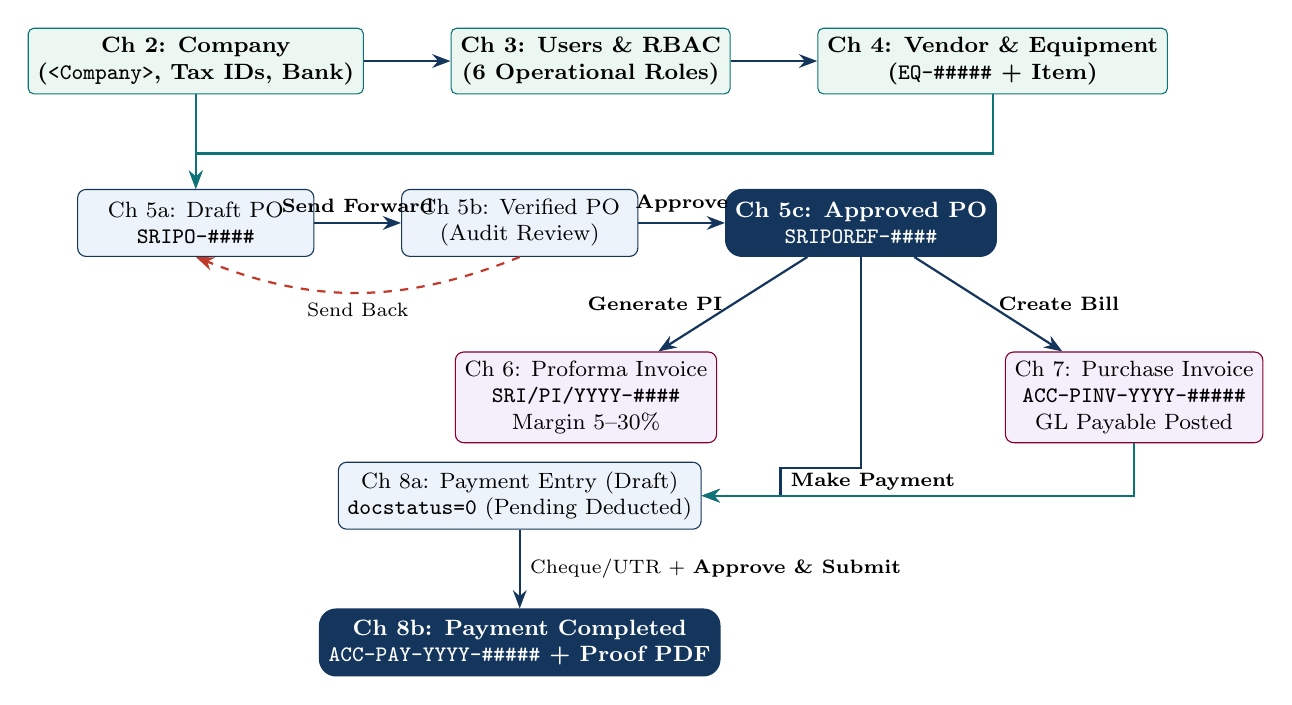
\begin{tikzpicture}[node distance=0.95cm and 1.1cm]
        % Row 1: Masters
        \node (co) [rolebox] {Ch 2: Company\\(\texttt{<Company>}, Tax IDs, Bank)};
        \node (usr) [rolebox, right=of co] {Ch 3: Users \& RBAC\\(6 Operational Roles)};
        \node (vnd) [rolebox, right=of usr] {Ch 4: Vendor \& Equipment\\(\texttt{EQ-\#\#\#\#\#} + Item)};

        % Row 2: PO Workflow
        \node (po1) [process, below=1.2cm of co] {Ch 5a: Draft PO\\\texttt{SRIPO-\#\#\#\#}};
        \node (po2) [process, right=of po1] {Ch 5b: Verified PO\\(Audit Review)};
        \node (po3) [startstop, right=of po2] {Ch 5c: Approved PO\\\texttt{SRIPOREF-\#\#\#\#}};

        % Row 3: Invoices
        \node (pi) [docnode, below left=1.2cm and 0.1cm of po3] {Ch 6: Proforma Invoice\\\texttt{SRI/PI/YYYY-\#\#\#\#}\\Margin 5--30\%};
        \node (pinv) [docnode, below right=1.2cm and 0.1cm of po3] {Ch 7: Purchase Invoice\\\texttt{ACC-PINV-YYYY-\#\#\#\#\#}\\GL Payable Posted};

        % Row 4: Payment Entry
        \node (ped) [process, below=2.6cm of po2] {Ch 8a: Payment Entry (Draft)\\\texttt{docstatus=0} (Pending Deducted)};
        \node (pes) [startstop, below=1.0cm of ped] {Ch 8b: Payment Completed\\\texttt{ACC-PAY-YYYY-\#\#\#\#\#} + Proof PDF};

        \draw [arrow] (co) -- (usr);
        \draw [arrow] (usr) -- (vnd);
        \draw [dataarrow] (co.south) -- (po1.north);
        \draw [dataarrow] (vnd.south) |- ($(po1.north)+(0,0.45)$) -| (po1.north);
        \draw [arrow] (po1) -- node[above, font=\scriptsize]{\textbf{Send Forward}} (po2);
        \draw [arrow] (po2) -- node[above, font=\scriptsize]{\textbf{Approve}} (po3);
        \draw [backarrow] (po2.south) to[bend left=22] node[below, font=\scriptsize]{Send Back} (po1.south);
        \draw [arrow] (po3) -- node[left, font=\scriptsize]{\textbf{Generate PI}} (pi);
        \draw [arrow] (po3) -- node[right, font=\scriptsize]{\textbf{Create Bill}} (pinv);
        \draw [arrow] (po3.south) |- ($(ped.east)+(1.0,0.35)$) |- (ped.east) node[pos=0.25, right, font=\scriptsize]{\textbf{Make Payment}};
        \draw [dataarrow] (pinv.south) |- (ped.east);
        \draw [arrow] (ped) -- node[right, font=\scriptsize]{Cheque/UTR + \textbf{Approve \& Submit}} (pes);
    \end{tikzpicture}}
    \caption{Master End-to-End Operational Lifecycle Flowchart}
    \label{fig:master-workflow}
\end{figure}

\section{Cross-Module Field Dataflow Diagram}

\begin{figure}[htbp]
    \centering
    \resizebox{!}{0.68\textheight}{%
    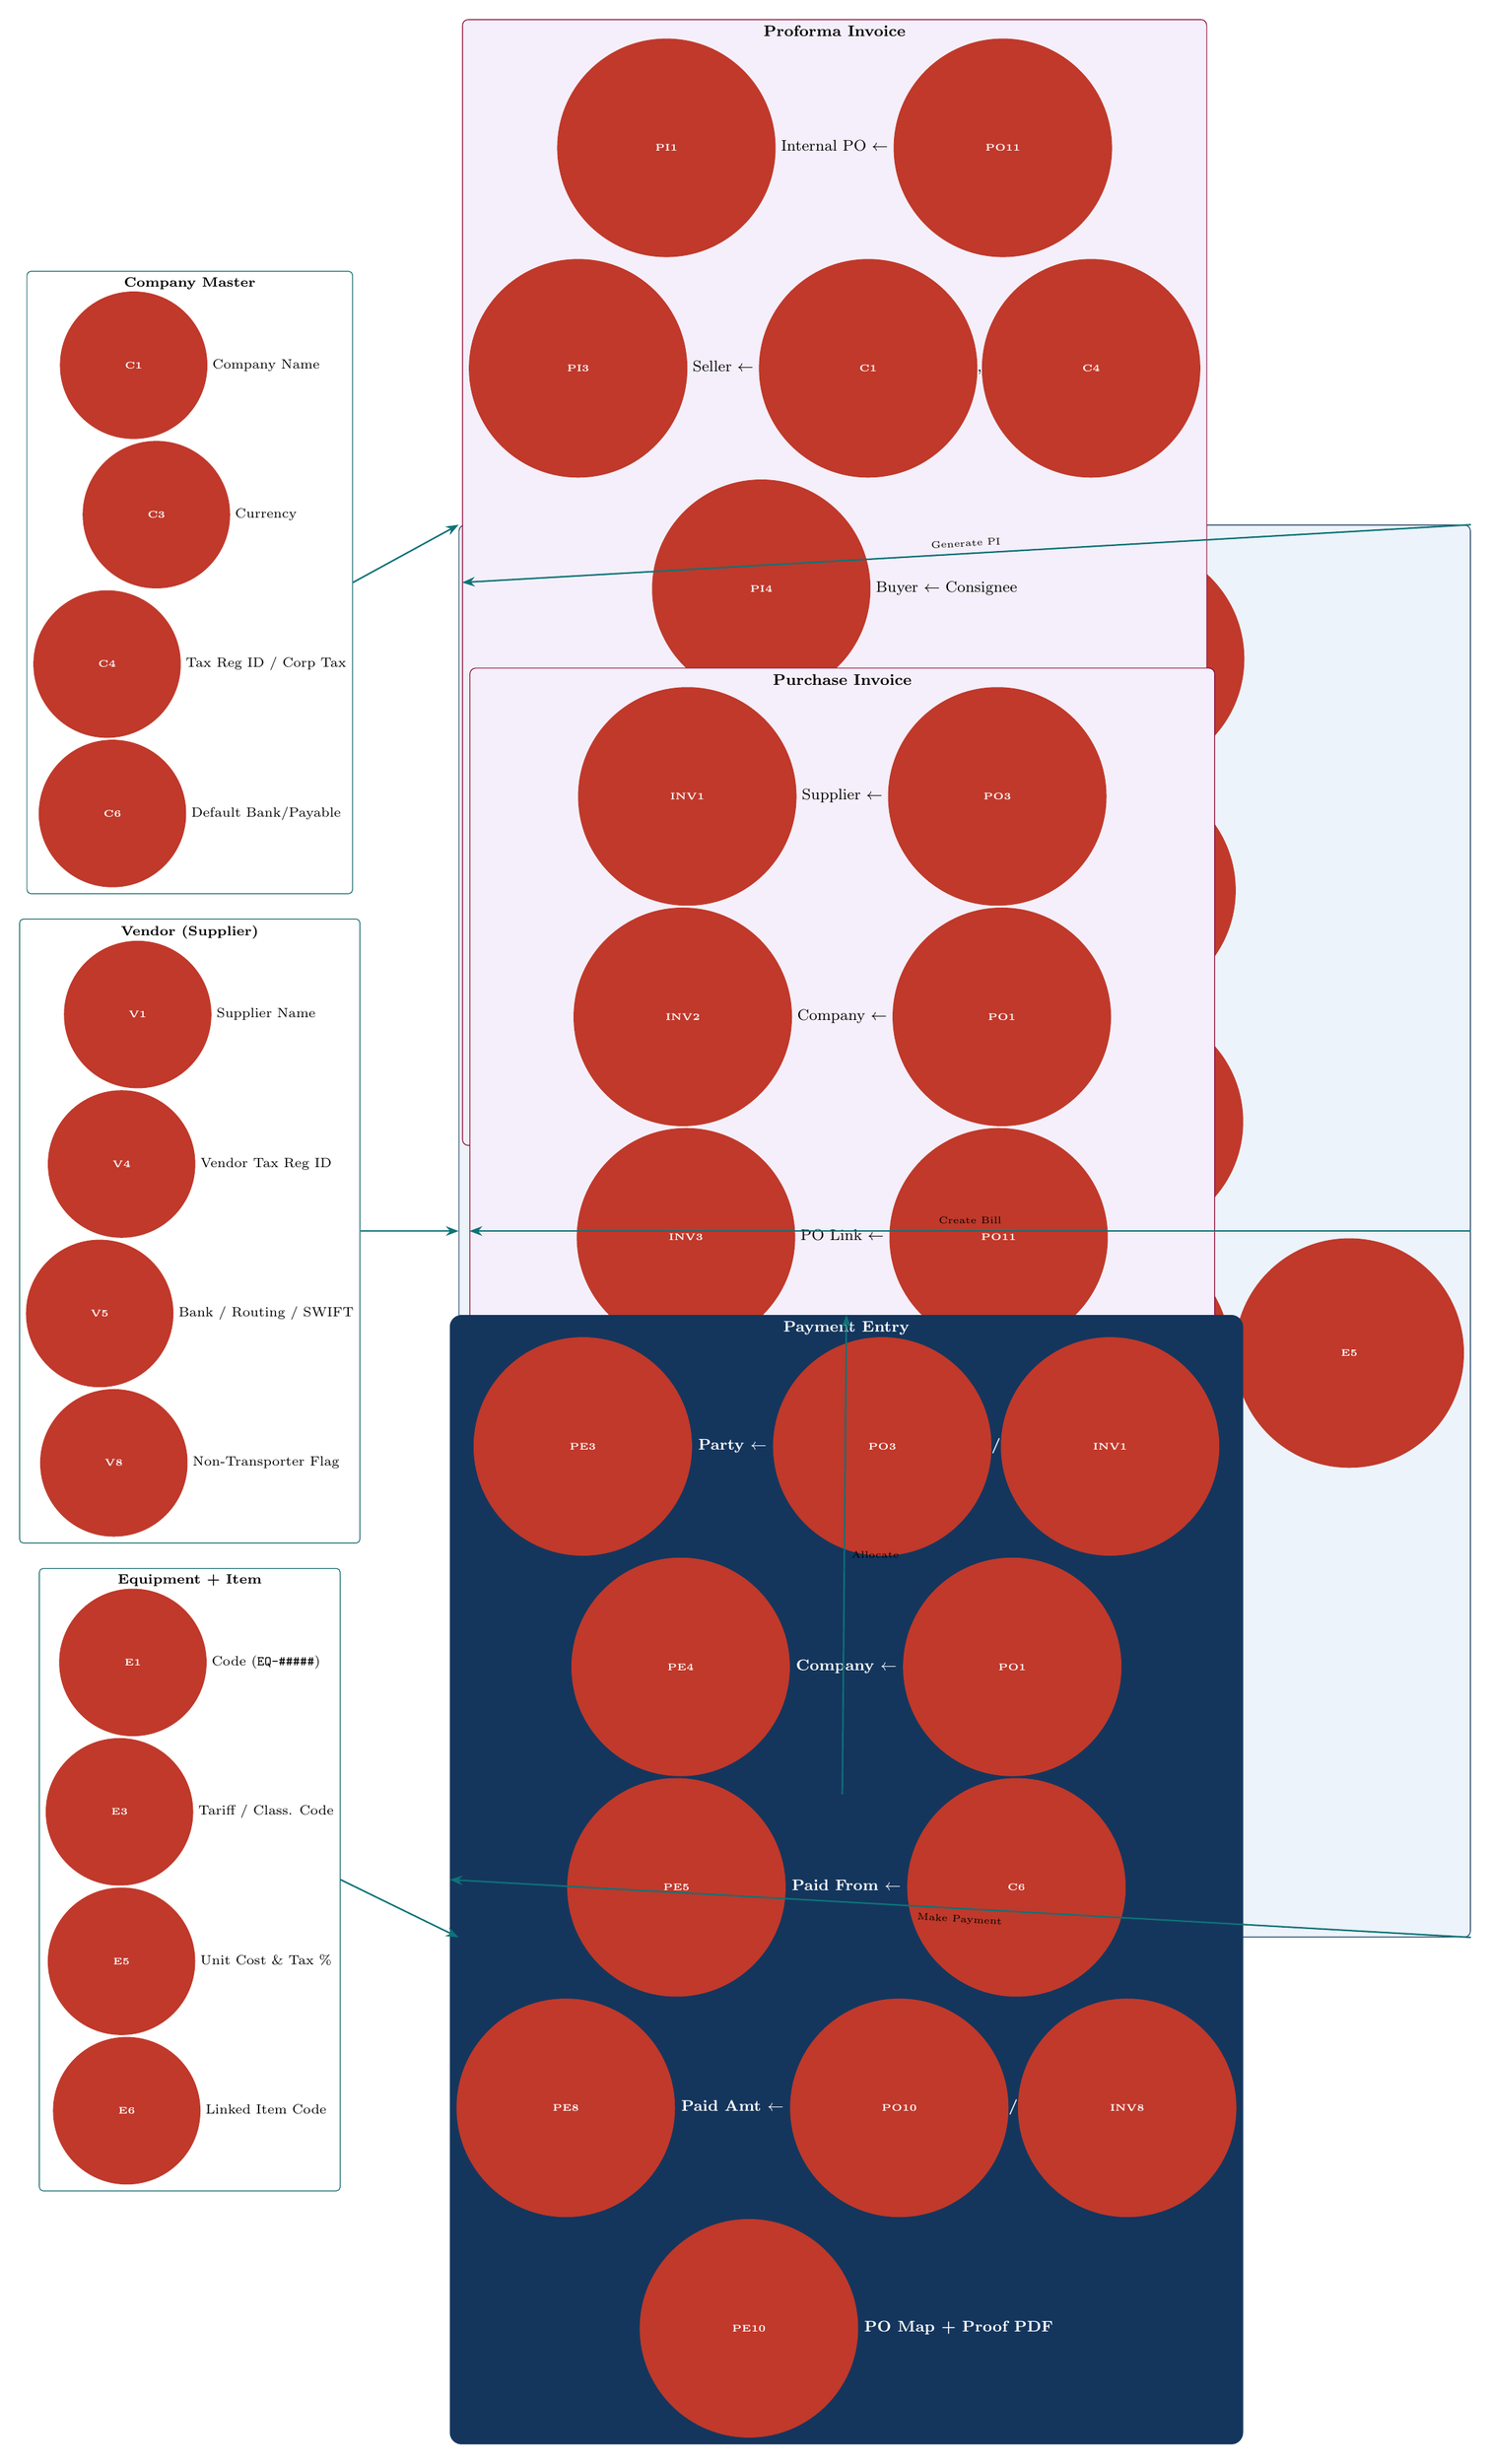
\begin{tikzpicture}[node distance=0.45cm and 0.9cm]
        \node (fco) [datanode] {\textbf{Company Master}\\
            \pin{C1} Company Name\\
            \pin{C3} Currency\\
            \pin{C4} Tax Reg ID / Corp Tax\\
            \pin{C6} Default Bank/Payable};

        \node (fv) [datanode, below=of fco] {\textbf{Vendor (Supplier)}\\
            \pin{V1} Supplier Name\\
            \pin{V4} Vendor Tax Reg ID\\
            \pin{V5} Bank / Routing / SWIFT\\
            \pin{V8} Non-Transporter Flag};

        \node (fe) [datanode, below=of fv] {\textbf{Equipment + Item}\\
            \pin{E1} Code (\texttt{EQ-\#\#\#\#\#})\\
            \pin{E3} Tariff / Class. Code\\
            \pin{E5} Unit Cost \& Tax \%\\
            \pin{E6} Linked Item Code};

        \node (fpo) [process, right=1.8cm of fv, minimum width=4.2cm] {\textbf{Vendor Purchase Order}\\
            \pin{PO1} Company $\leftarrow$ \pin{C1}\\
            \pin{PO3} Vendor $\leftarrow$ \pin{V1}\\
            \pin{PO4} Currency $\leftarrow$ \pin{C3}\\
            \pin{PO6} Items $\leftarrow$ \pin{E1},\pin{E3},\pin{E5}\\
            \pin{PO8} Grand Total \& Tax\\
            \pin{PO10} Advance \& Schedule};

        \node (fpi) [docnode, right=2.0cm of fco, minimum width=4.0cm] {\textbf{Proforma Invoice}\\
            \pin{PI1} Internal PO $\leftarrow$ \pin{PO11}\\
            \pin{PI3} Seller $\leftarrow$ \pin{C1},\pin{C4}\\
            \pin{PI4} Buyer $\leftarrow$ Consignee\\
            \pin{PI6} Base + Margin (5--30\%)\\
            \pin{PI9} Beneficiary Bank $\leftarrow$ \pin{C6}};

        \node (finv) [docnode, right=2.0cm of fv, minimum width=4.0cm] {\textbf{Purchase Invoice}\\
            \pin{INV1} Supplier $\leftarrow$ \pin{PO3}\\
            \pin{INV2} Company $\leftarrow$ \pin{PO1}\\
            \pin{INV3} PO Link $\leftarrow$ \pin{PO11}\\
            \pin{INV6} Items $\leftarrow$ \pin{E6},\pin{PO6}\\
            \pin{INV8} Schedule $\leftarrow$ \pin{PO10}};

        \node (fpe) [startstop, right=2.0cm of fe, minimum width=4.0cm] {\textbf{Payment Entry}\\
            \pin{PE3} Party $\leftarrow$ \pin{PO3}/\pin{INV1}\\
            \pin{PE4} Company $\leftarrow$ \pin{PO1}\\
            \pin{PE5} Paid From $\leftarrow$ \pin{C6}\\
            \pin{PE8} Paid Amt $\leftarrow$ \pin{PO10}/\pin{INV8}\\
            \pin{PE10} PO Map + Proof PDF};

        \draw [dataarrow] (fco.east) -- (fpo.north west);
        \draw [dataarrow] (fv.east) -- (fpo.west);
        \draw [dataarrow] (fe.east) -- (fpo.south west);

        \draw [dataarrow] (fpo.north east) -- node[above, sloped, font=\tiny]{Generate PI} (fpi.west);
        \draw [dataarrow] (fpo.east) -- node[above, font=\tiny]{Create Bill} (finv.west);
        \draw [dataarrow] (fpo.south east) -- node[below, sloped, font=\tiny]{Make Payment} (fpe.west);
        \draw [dataarrow] (finv.south) -- node[right, font=\tiny]{Allocate} (fpe.north);
    \end{tikzpicture}}
    \caption{Master Field-Level Dataflow Diagram Across ERP Modules}
    \label{fig:master-dataflow}
\end{figure}

\begin{table}[htbp]
    \centering
    \caption{Deployed Document Numbering Standards}
    \label{tab:numbering}
    \begin{tabularx}{\textwidth}{l l l X}
        \toprule
        \textbf{Document} & \textbf{Naming Format} & \textbf{Placeholder Example} & \textbf{Trigger} \\
        \midrule
        Equipment\index{Equipment!Code} & \texttt{EQ-\#\#\#\#\#} & \texttt{EQ-XXXXX} & On Save \\
        Vendor PO\index{Purchase Order!Numbering} & \texttt{SRIPO-\#\#\#\#} & \texttt{SRIPO-XXXX} & On initial Draft Save \\
        PO Approval Ref\index{Purchase Order!Reference Number} & \texttt{SRIPOREF-\#\#\#\#} & \texttt{SRIPOREF-XXXX} & On Workflow \textbf{Approved} \\
        Proforma Invoice\index{Proforma Invoice!Numbering} & \texttt{SRI/PI/YYYY-\#\#\#\#} & \texttt{SRI/PI/YYYY-XXXX} & On Save from Approved PO \\
        Purchase Invoice\index{Purchase Invoice!Numbering} & \texttt{ACC-PINV-YYYY-\#\#\#\#\#} & \texttt{ACC-PINV-YYYY-XXXXX} & On \textbf{Create Bill} \\
        Payment Entry\index{Payment Entry!Numbering} & \texttt{ACC-PAY-YYYY-\#\#\#\#\#} & \texttt{ACC-PAY-YYYY-XXXXX} & On \textbf{Make Payment} / Save \\
        \bottomrule
    \end{tabularx}
\end{table}

% -------------------------------------------------------------------------
% CHAPTER 2: COMPANY MASTER
% -------------------------------------------------------------------------
\chapter{Preparing the Company Master}
\index{Company!Setup}\index{Company!Tax IDs}\index{Company!Bank Account}

\section{Company Configuration \& Tax Rule Flowchart}

\begin{figure}[htbp]
    \centering
    \resizebox{\textwidth}{!}{%
    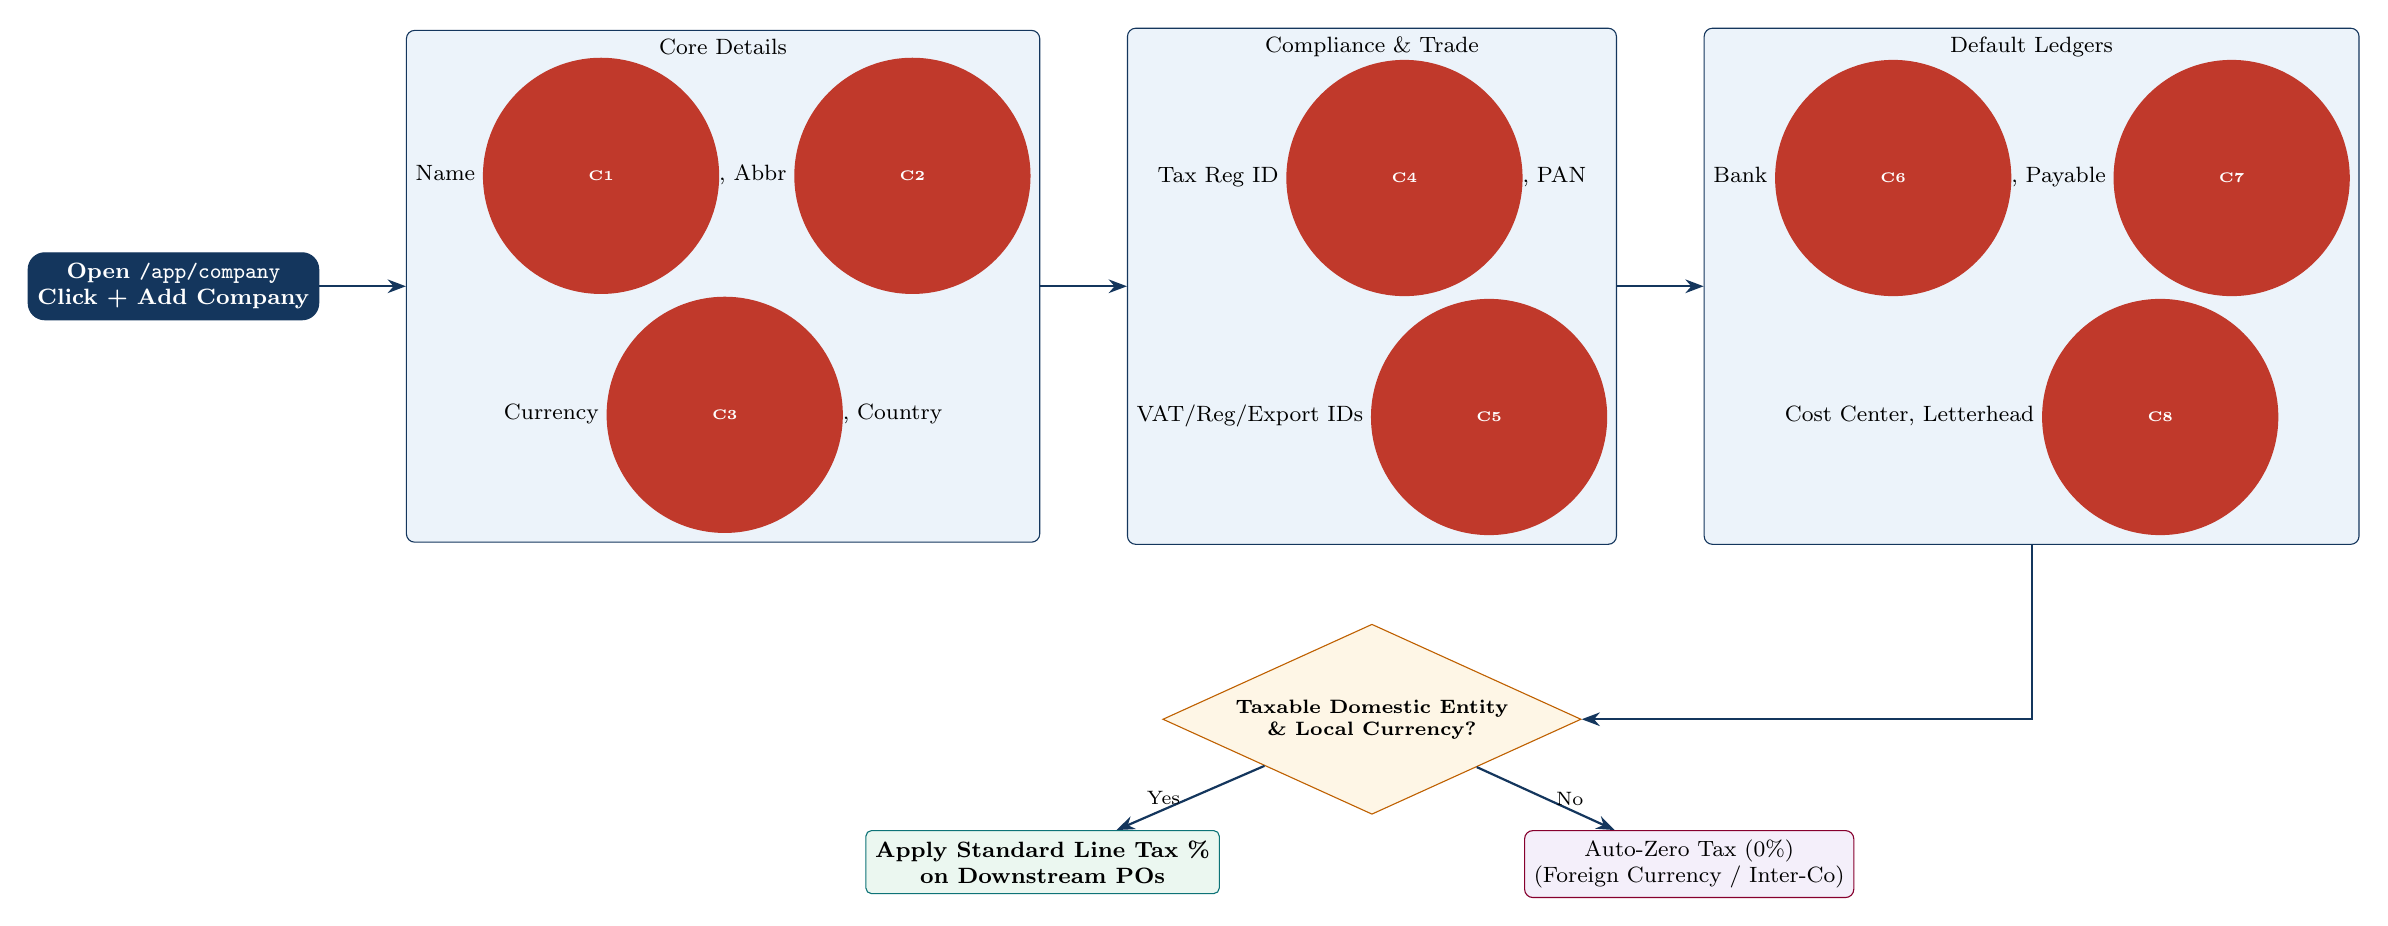
\begin{tikzpicture}[node distance=0.85cm and 1.1cm]
        \node (cstart) [startstop] {Open \texttt{/app/company}\\Click \textbf{+ Add Company}};
        \node (cstep1) [process, right=of cstart] {Core Details\\Name \pin{C1}, Abbr \pin{C2}\\Currency \pin{C3}, Country};
        \node (cstep2) [process, right=of cstep1] {Compliance \& Trade\\Tax Reg ID \pin{C4}, PAN\\VAT/Reg/Export IDs \pin{C5}};
        \node (cstep3) [process, right=of cstep2] {Default Ledgers\\Bank \pin{C6}, Payable \pin{C7}\\Cost Center, Letterhead \pin{C8}};
        \node (cdec) [decision, below=1.0cm of cstep2] {Taxable Domestic Entity\\\& Local Currency?};
        \node (ctax) [rolebox, below left=0.8cm and 0.6cm of cdec] {Apply Standard Line Tax \%\\on Downstream POs};
        \node (cexempt) [docnode, below right=0.8cm and 0.6cm of cdec] {Auto-Zero Tax (0\%)\\(Foreign Currency / Inter-Co)};

        \draw [arrow] (cstart) -- (cstep1);
        \draw [arrow] (cstep1) -- (cstep2);
        \draw [arrow] (cstep2) -- (cstep3);
        \draw [arrow] (cstep3.south) |- (cdec.east);
        \draw [arrow] (cdec) -- node[left, font=\scriptsize]{Yes} (ctax);
        \draw [arrow] (cdec) -- node[right, font=\scriptsize]{No} (cexempt);
    \end{tikzpicture}}
    \caption{Company Preparation and Automatic Tax Rule Decision Flow}
    \label{fig:company-flow}
\end{figure}

\section{Website Screenshot Layout \& Marked Fields (\texttt{Company})}

\begin{webframe}{company/<Company-Name>}{Actual Website Screen: Company Form}
\centering
\resizebox{0.97\textwidth}{!}{%
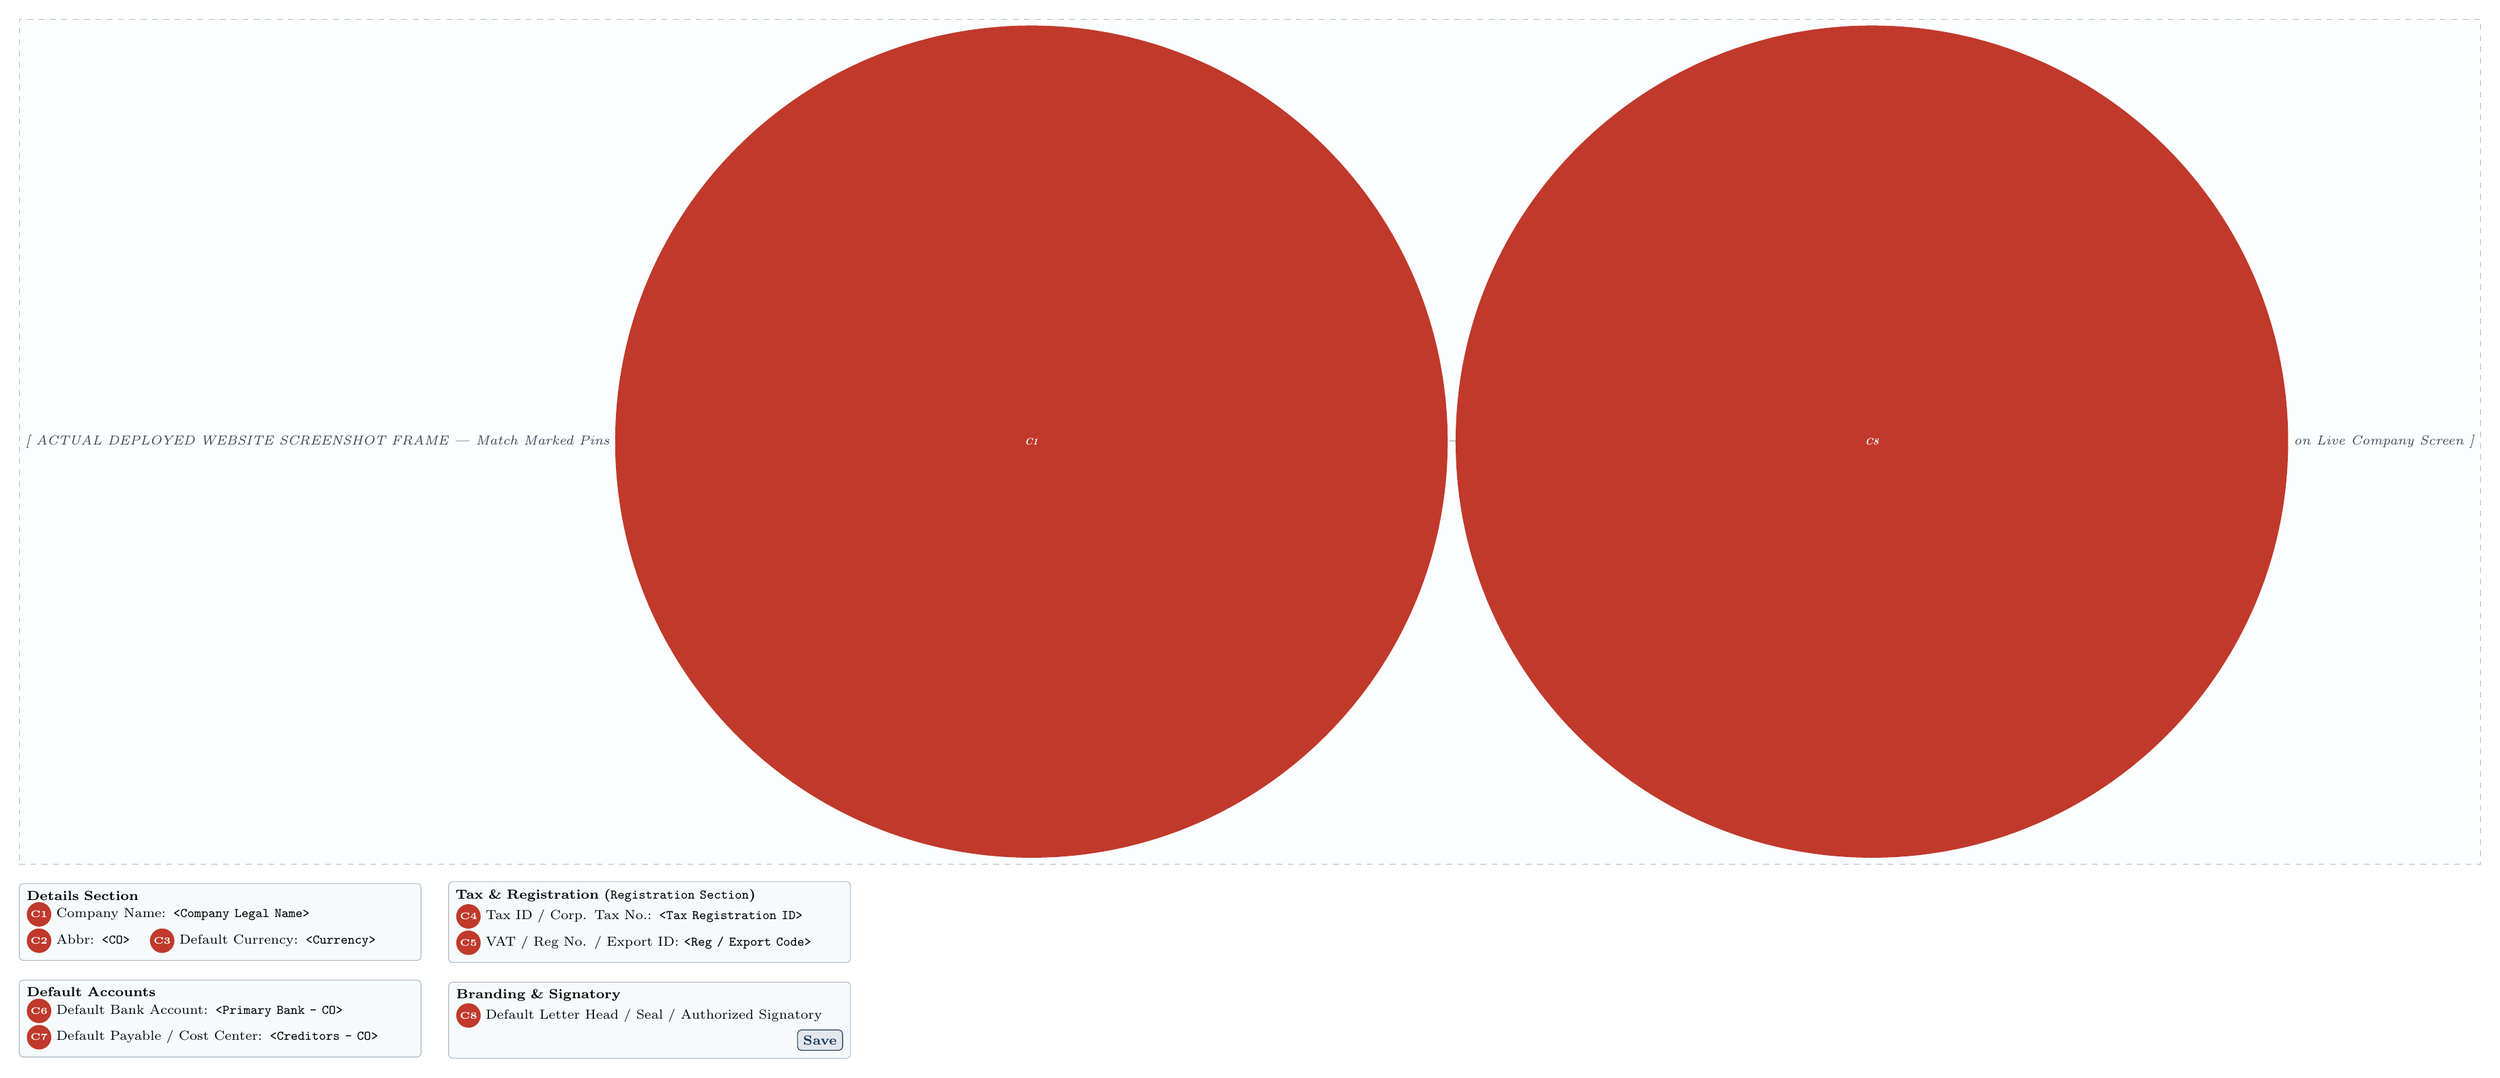
\begin{tikzpicture}[node distance=0.35cm and 0.45cm]
    \node[draw=bordergray, dashed, fill=softblue!20, minimum width=15.5cm, minimum height=0.6cm, font=\scriptsize\itshape, text=darkgray] (banner) at (0,0)
        {[ ACTUAL DEPLOYED WEBSITE SCREENSHOT FRAME --- Match Marked Pins \pin{C1}--\pin{C8} on Live Company Screen ]};

    \node[uibox, text width=7.2cm, below=0.35cm of banner.south west, anchor=north west] (sec1) {
        \textbf{Details Section}\\
        \pin{C1} Company Name: \texttt{<Company Legal Name>}\\
        \pin{C2} Abbr: \texttt{<CO>} \quad \pin{C3} Default Currency: \texttt{<Currency>}
    };
    \node[uibox, text width=7.2cm, right=0.5cm of sec1] (sec2) {
        \textbf{Tax \& Registration (\texttt{Registration Section})}\\
        \pin{C4} Tax ID / Corp. Tax No.: \texttt{<Tax Registration ID>}\\
        \pin{C5} VAT / Reg No. / Export ID: \texttt{<Reg / Export Code>}
    };
    \node[uibox, text width=7.2cm, below=0.35cm of sec1] (sec3) {
        \textbf{Default Accounts}\\
        \pin{C6} Default Bank Account: \texttt{<Primary Bank - CO>}\\
        \pin{C7} Default Payable / Cost Center: \texttt{<Creditors - CO>}
    };
    \node[uibox, text width=7.2cm, below=0.35cm of sec2] (sec4) {
        \textbf{Branding \& Signatory}\\
        \pin{C8} Default Letter Head / Seal / Authorized Signatory\\
        \hfill \tikz\node[uibtn]{Save};
    };
\end{tikzpicture}}
\end{webframe}

\begin{table}[htbp]
    \centering
    \caption{Company Field Markings \& Downstream Dataflow}
    \label{tab:company-fields}
    \begin{tabularx}{\textwidth}{c l l X}
        \toprule
        \textbf{Pin} & \textbf{Website UI Field} & \textbf{Generic Value} & \textbf{Dataflow Propagation} \\
        \midrule
        \pin{C1} & Company Name & \texttt{<Company Legal Name>} & Populates PO \pin{PO1}, PI Seller \pin{PI3}, Bill \pin{INV2}, PE \pin{PE4} \\
        \pin{C2} & Abbr & \texttt{<CO>} & Appends ledger suffix on Bank/Creditors/Cost Centers \\
        \pin{C3} & Default Currency & \texttt{<Currency>} & Drives tax applicability \& exchange-rate logic \\
        \pin{C4} & Tax ID / Corporate Tax ID & \texttt{<Tax Registration ID>} & Auto-copied onto Vendor PO \& Proforma Invoice headers \\
        \pin{C5} & VAT / Company Reg / Export ID & \texttt{<Reg / Export Code>} & Auto-copied to PI Seller trade compliance block \\
        \pin{C6} & Default Bank Account & \texttt{<Primary Bank - CO>} & Pre-selected as \textbf{Paid From} \pin{PE5} on Payment Entries \\
        \pin{C7} & Default Payable Account & \texttt{<Creditors - CO>} & Auto-linked as \textbf{Paid To} / Liability account \\
        \pin{C8} & Letterhead / Seal / Signatory & \texttt{<Official Template>} & Rendered onto printed PO, PI, and Payment Proof PDFs \\
        \bottomrule
    \end{tabularx}
\end{table}

% -------------------------------------------------------------------------
% CHAPTER 3: USERS & ROLES
% -------------------------------------------------------------------------
\chapter{Preparing Users and Role Permissions}
\index{User!Creation}\index{Roles and Permissions}

\section{Role Segregation \& Action Gate Flowchart}

\begin{figure}[htbp]
    \centering
    \resizebox{\textwidth}{!}{%
    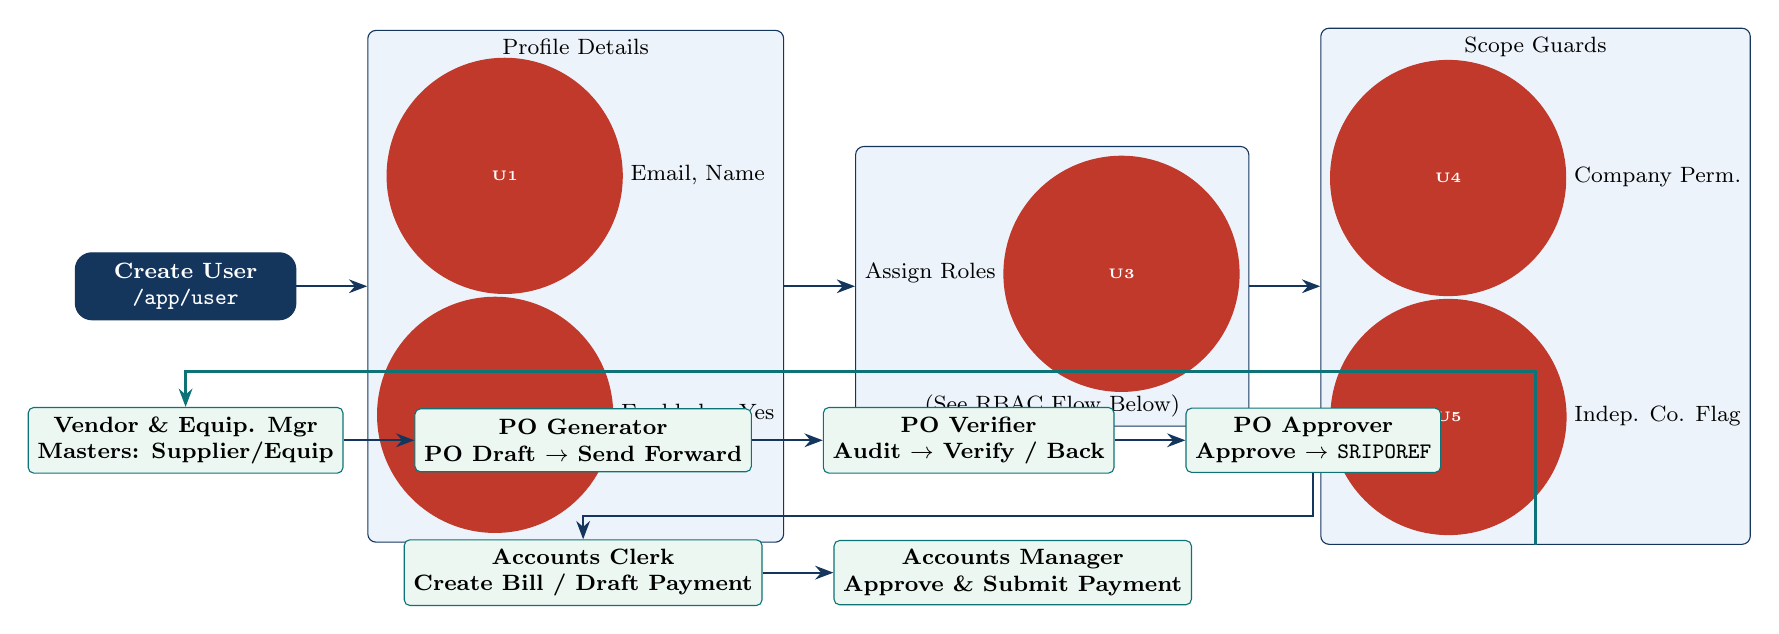
\begin{tikzpicture}[node distance=0.85cm and 0.9cm]
        \node (uadd) [startstop] {Create User\\\texttt{/app/user}};
        \node (uprof) [process, right=of uadd] {Profile Details\\\pin{U1} Email, Name\\\pin{U2} Enabled = Yes};
        \node (urole) [process, right=of uprof] {Assign Roles \pin{U3}\\(See RBAC Flow Below)};
        \node (uperm) [process, right=of urole] {Scope Guards\\\pin{U4} Company Perm.\\\pin{U5} Indep. Co. Flag};

        % RBAC swimlane
        \node (r0) [rolebox, below=1.1cm of uadd] {\textbf{Vendor \& Equip. Mgr}\\Masters: Supplier/Equip};
        \node (r1) [rolebox, right=of r0] {\textbf{PO Generator}\\PO Draft $\rightarrow$ \textbf{Send Forward}};
        \node (r2) [rolebox, right=of r1] {\textbf{PO Verifier}\\Audit $\rightarrow$ \textbf{Verify} / Back};
        \node (r3) [rolebox, right=of r2] {\textbf{PO Approver}\\\textbf{Approve} $\rightarrow$ \texttt{SRIPOREF}};
        \node (r4) [rolebox, below=0.85cm of r1] {\textbf{Accounts Clerk}\\\textbf{Create Bill} / Draft Payment};
        \node (r5) [rolebox, right=of r4] {\textbf{Accounts Manager}\\\textbf{Approve \& Submit} Payment};

        \draw [arrow] (uadd) -- (uprof);
        \draw [arrow] (uprof) -- (urole);
        \draw [arrow] (urole) -- (uperm);
        \draw [dataarrow] (uperm.south) |- ($(r0.north)+(0,0.45)$) -| (r0.north);
        \draw [arrow] (r0) -- (r1);
        \draw [arrow] (r1) -- (r2);
        \draw [arrow] (r2) -- (r3);
        \draw [arrow] (r3.south) |- ($(r4.north)+(0,0.3)$) -| (r4.north);
        \draw [arrow] (r4) -- (r5);
    \end{tikzpicture}}
    \caption{User Provisioning and Role-Based Action Gate Workflow}
    \label{fig:rbac-flow}
\end{figure}

\section{Website Screenshot Layout \& Marked Fields (\texttt{User})}

\begin{webframe}{user/<User-Email>}{Actual Website Screen: User \& Roles Form}
\centering
\resizebox{0.97\textwidth}{!}{%
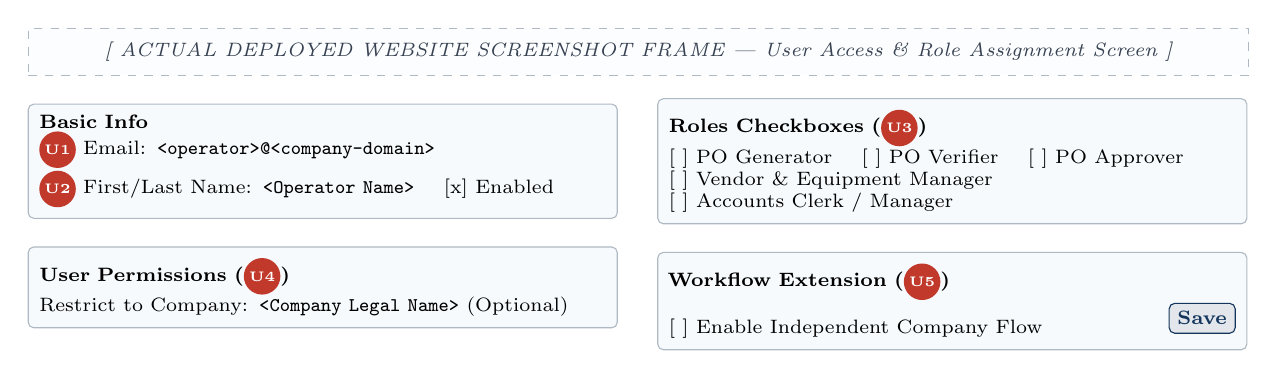
\begin{tikzpicture}[node distance=0.35cm and 0.45cm]
    \node[draw=bordergray, dashed, fill=softblue!20, minimum width=15.5cm, minimum height=0.6cm, font=\scriptsize\itshape, text=darkgray] (ubanner) at (0,0)
        {[ ACTUAL DEPLOYED WEBSITE SCREENSHOT FRAME --- User Access \& Role Assignment Screen ]};

    \node[uibox, text width=7.2cm, below=0.35cm of ubanner.south west, anchor=north west] (usec1) {
        \textbf{Basic Info}\\
        \pin{U1} Email: \texttt{<operator>@<company-domain>}\\
        \pin{U2} First/Last Name: \texttt{<Operator Name>} \quad \mbox{[x] Enabled}
    };
    \node[uibox, text width=7.2cm, right=0.5cm of usec1] (usec2) {
        \textbf{Roles Checkboxes (\pin{U3})}\\
        \mbox{[ ] PO Generator} \quad \mbox{[ ] PO Verifier} \quad \mbox{[ ] PO Approver}\\
        \mbox{[ ] Vendor \& Equipment Manager} \quad \mbox{[ ] Accounts Clerk / Manager}
    };
    \node[uibox, text width=7.2cm, below=0.35cm of usec1] (usec3) {
        \textbf{User Permissions (\pin{U4})}\\
        Restrict to Company: \texttt{<Company Legal Name>} (Optional)
    };
    \node[uibox, text width=7.2cm, below=0.35cm of usec2] (usec4) {
        \textbf{Workflow Extension (\pin{U5})}\\
        \mbox{[ ] Enable Independent Company Flow} \hfill \tikz\node[uibtn]{Save};
    };
\end{tikzpicture}}
\end{webframe}

\begin{cautionbox}{Permission Enforcement Rule}
Action buttons (\textbf{Send Forward}, \textbf{Create Bill}, \textbf{Make Payment}, \textbf{Approve \& Submit}) stay hidden if the logged-in user lacks the matching role in \pin{U3}.
\end{cautionbox}

% -------------------------------------------------------------------------
% CHAPTER 4: VENDOR & EQUIPMENT
% -------------------------------------------------------------------------
\chapter{Preparing Vendors and Equipment Masters}
\index{Vendor!Setup}\index{Equipment!Setup}\index{Supplier|see{Vendor}}

\section{Vendor \& Equipment Dataflow to Procurement}

\begin{figure}[htbp]
    \centering
    \resizebox{\textwidth}{!}{%
    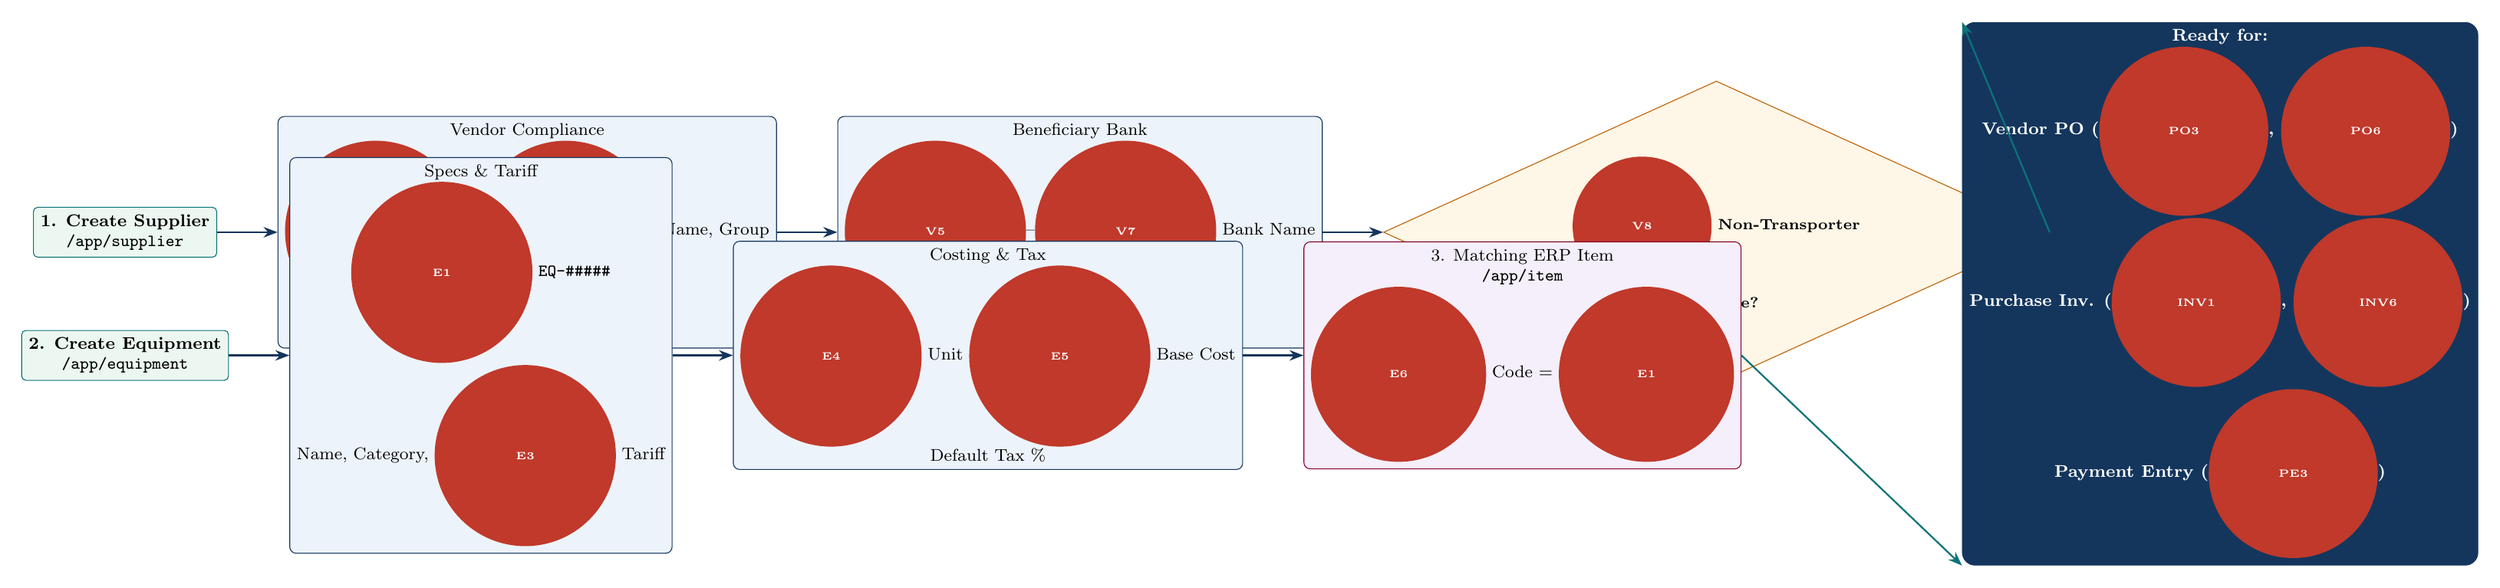
\begin{tikzpicture}[node distance=0.8cm and 1.0cm]
        \node (v1) [rolebox] {1. Create Supplier\\\texttt{/app/supplier}};
        \node (v2) [process, right=of v1] {Vendor Compliance\\\pin{V1}--\pin{V4} Name, Group\\Tax Reg ID, Tax/WHT \%};
        \node (v3) [process, right=of v2] {Beneficiary Bank\\\pin{V5}--\pin{V7} Bank Name\\Acct No., Routing/SWIFT};
        \node (v4) [decision, right=of v3] {\pin{V8} Non-Transporter\\\& Active?};

        \node (e1) [rolebox, below=1.2cm of v1] {2. Create Equipment\\\texttt{/app/equipment}};
        \node (e2) [process, right=of e1] {Specs \& Tariff\\\pin{E1} \texttt{EQ-\#\#\#\#\#}\\Name, Category, \pin{E3} Tariff};
        \node (e3) [process, right=of e2] {Costing \& Tax\\\pin{E4} Unit \pin{E5} Base Cost\\Default Tax \%};
        \node (e4) [docnode, right=of e3] {3. Matching ERP Item\\\texttt{/app/item}\\\pin{E6} Code = \pin{E1}};

        \node (target) [startstop, right=1.1cm of $(v4.east)!0.5!(e4.east)$, minimum height=1.8cm] {Ready for:\\Vendor PO (\pin{PO3}, \pin{PO6})\\Purchase Inv. (\pin{INV1}, \pin{INV6})\\Payment Entry (\pin{PE3})};

        \draw [arrow] (v1) -- (v2);
        \draw [arrow] (v2) -- (v3);
        \draw [arrow] (v3) -- (v4);
        \draw [dataarrow] (v4.east) -- (target.north west);

        \draw [arrow] (e1) -- (e2);
        \draw [arrow] (e2) -- (e3);
        \draw [arrow] (e3) -- (e4);
        \draw [dataarrow] (e4.east) -- (target.south west);
    \end{tikzpicture}}
    \caption{Vendor, Equipment, and Matching Item Synchronization Dataflow}
    \label{fig:vendor-equip-dataflow}
\end{figure}

\section{Website Screenshot Layout \& Marked Fields (\texttt{Supplier} \& \texttt{Equipment})}

\begin{webframe}{supplier / equipment}{Actual Website Screens: Vendor \& Equipment Forms}
\centering
\resizebox{0.97\textwidth}{!}{%
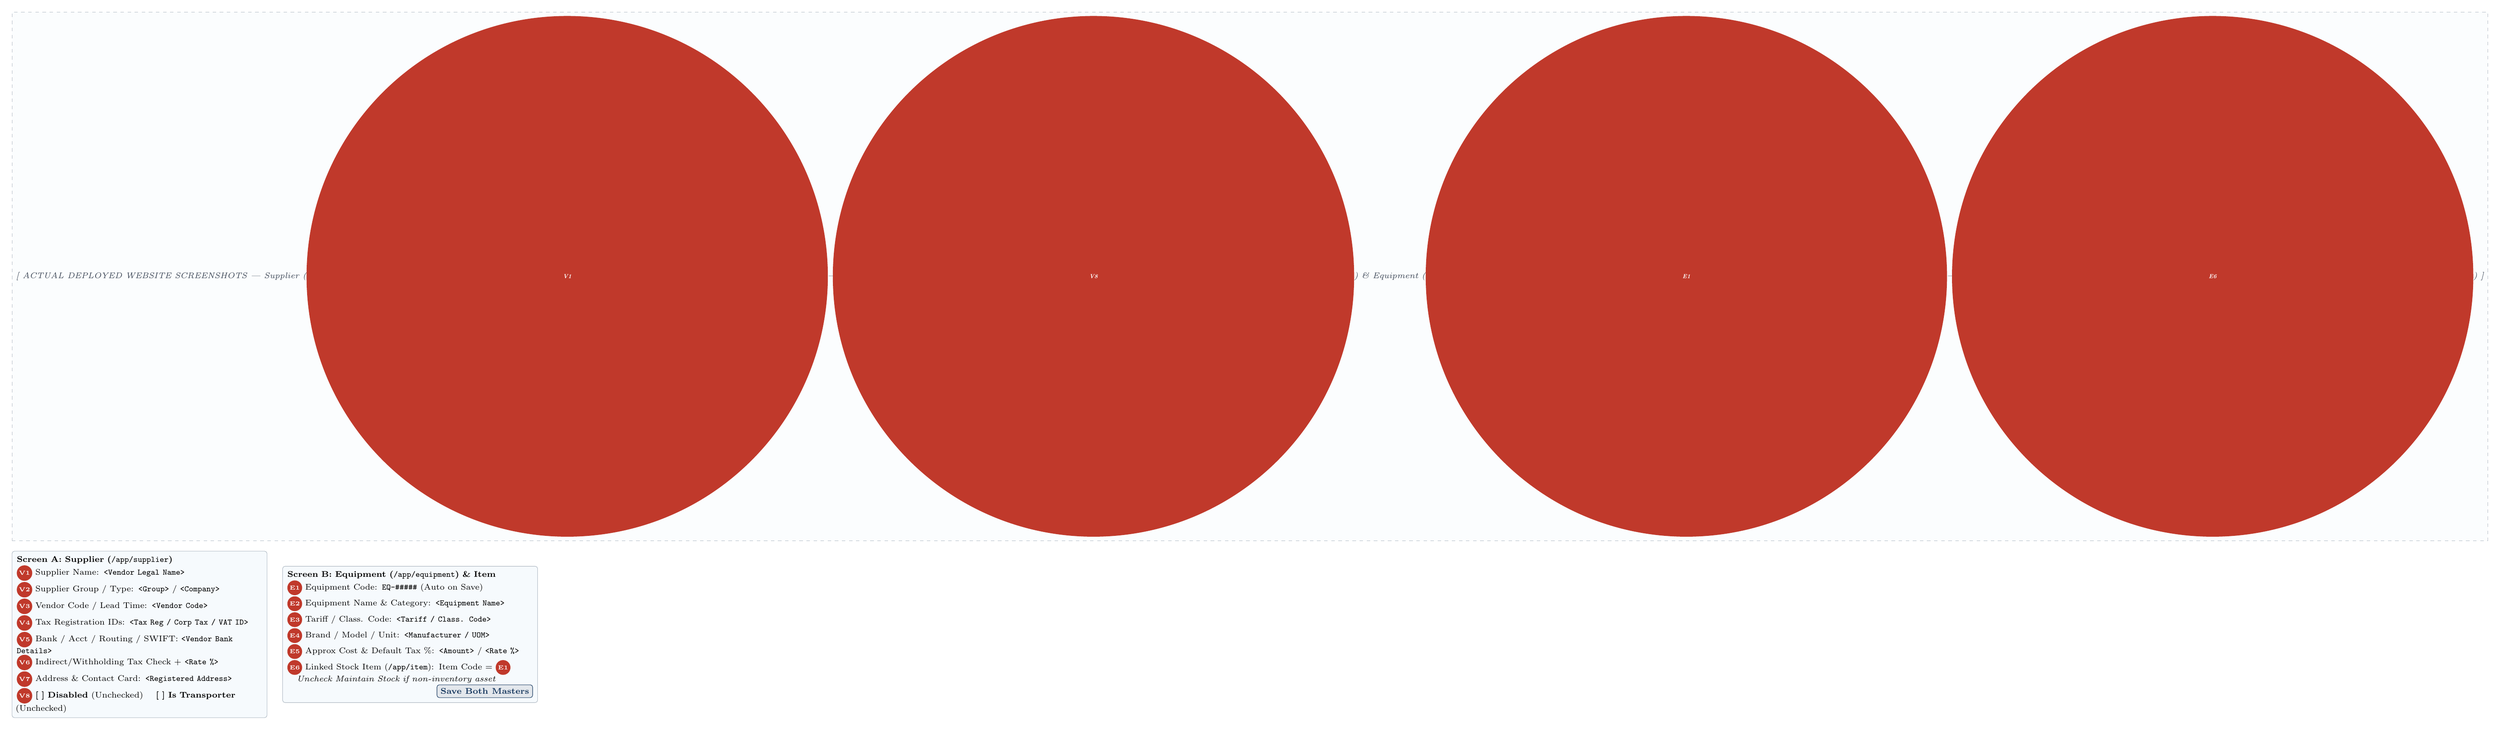
\begin{tikzpicture}[node distance=0.35cm and 0.45cm]
    \node[draw=bordergray, dashed, fill=softblue!20, minimum width=15.5cm, minimum height=0.55cm, font=\scriptsize\itshape, text=darkgray] (vbanner) at (0,0)
        {[ ACTUAL DEPLOYED WEBSITE SCREENSHOTS --- Supplier (\pin{V1}--\pin{V8}) \& Equipment (\pin{E1}--\pin{E6}) ]};

    \node[uibox, text width=7.3cm, below=0.3cm of vbanner.south west, anchor=north west] (vui) {
        \textbf{Screen A: Supplier (\texttt{/app/supplier})}\\
        \pin{V1} Supplier Name: \texttt{<Vendor Legal Name>}\\
        \pin{V2} Supplier Group / Type: \texttt{<Group>} / \texttt{<Company>}\\
        \pin{V3} Vendor Code / Lead Time: \texttt{<Vendor Code>}\\
        \pin{V4} Tax Registration IDs: \texttt{<Tax Reg / Corp Tax / VAT ID>}\\
        \pin{V5} Bank / Acct / Routing / SWIFT: \texttt{<Vendor Bank Details>}\\
        \pin{V6} Indirect/Withholding Tax Check + \texttt{<Rate \%>}\\
        \pin{V7} Address \& Contact Card: \texttt{<Registered Address>}\\
        \pin{V8} \textbf{\mbox{[ ] Disabled}} (Unchecked) \quad \textbf{\mbox{[ ] Is Transporter}} (Unchecked)
    };
    \node[uibox, text width=7.3cm, right=0.45cm of vui] (eui) {
        \textbf{Screen B: Equipment (\texttt{/app/equipment}) \& Item}\\
        \pin{E1} Equipment Code: \texttt{EQ-\#\#\#\#\#} (Auto on Save)\\
        \pin{E2} Equipment Name \& Category: \texttt{<Equipment Name>}\\
        \pin{E3} Tariff / Class. Code: \texttt{<Tariff / Class. Code>}\\
        \pin{E4} Brand / Model / Unit: \texttt{<Manufacturer / UOM>}\\
        \pin{E5} Approx Cost \& Default Tax \%: \texttt{<Amount>} / \texttt{<Rate \%>}\\
        \pin{E6} Linked Stock Item (\texttt{/app/item}): Item Code = \pin{E1}\\
        \quad \textit{Uncheck Maintain Stock if non-inventory asset}\\
        \hfill \tikz\node[uibtn]{Save Both Masters};
    };
\end{tikzpicture}}
\end{webframe}

\begin{rulebox}{Transporter Filter \& Dual Master Sync}
\begin{itemize}[leftmargin=1.5em, itemsep=1pt]
    \item Keep \pin{V8} \textbf{Is Transporter} unchecked; transporter records are filtered out of Payment Entry lookups.
    \item Match \textbf{Item Code} (\pin{E6}) to \textbf{Equipment Code} (\pin{E1}) so Purchase Invoices auto-map PO items cleanly.
\end{itemize}
\end{rulebox}

% -------------------------------------------------------------------------
% CHAPTER 5: VENDOR PURCHASE ORDER
% -------------------------------------------------------------------------
\chapter{Preparing and Approving a Purchase Order}
\index{Purchase Order!Creation}\index{Purchase Order!Approval Workflow}\index{Payment Order|see{Purchase Order}}

\section{Three-Stage PO Approval Workflow Flowchart}

\begin{figure}[htbp]
    \centering
    \resizebox{\textwidth}{!}{%
    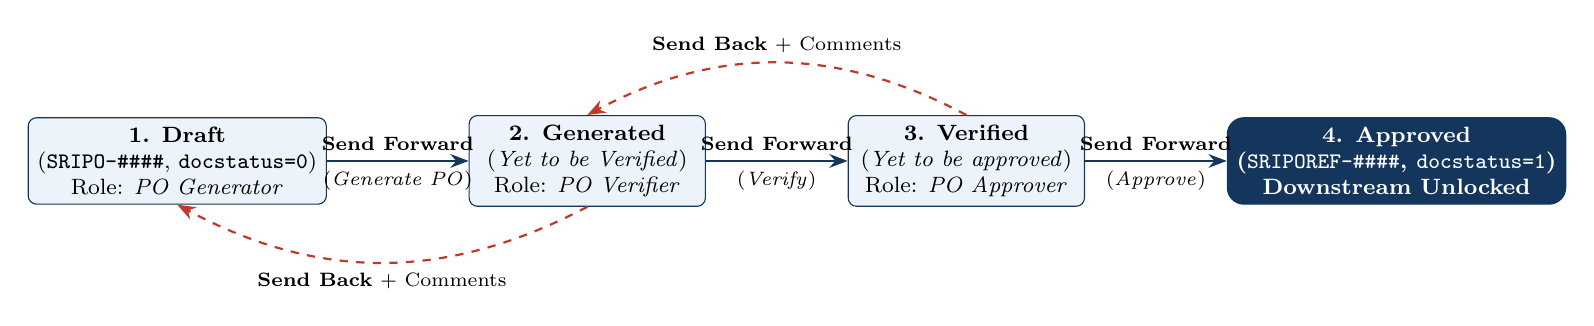
\begin{tikzpicture}[node distance=1.0cm and 1.35cm]
        \node (draft) [process] {\textbf{1. Draft}\\(\texttt{SRIPO-\#\#\#\#}, \texttt{docstatus=0})\\Role: \textit{PO Generator}};
        \node (gen) [process, right=1.8cm of draft] {\textbf{2. Generated}\\(\textit{Yet to be Verified})\\Role: \textit{PO Verifier}};
        \node (ver) [process, right=1.8cm of gen] {\textbf{3. Verified}\\(\textit{Yet to be approved})\\Role: \textit{PO Approver}};
        \node (app) [startstop, right=1.8cm of ver] {\textbf{4. Approved}\\(\texttt{SRIPOREF-\#\#\#\#}, \texttt{docstatus=1})\\Downstream Unlocked};

        \draw [arrow] (draft) -- node[above, font=\scriptsize]{\textbf{Send Forward}} node[below, font=\scriptsize]{(\textit{Generate PO})} (gen);
        \draw [arrow] (gen) -- node[above, font=\scriptsize]{\textbf{Send Forward}} node[below, font=\scriptsize]{(\textit{Verify})} (ver);
        \draw [arrow] (ver) -- node[above, font=\scriptsize]{\textbf{Send Forward}} node[below, font=\scriptsize]{(\textit{Approve})} (app);

        \draw [backarrow] (gen.south) to[bend left=28] node[below, font=\scriptsize]{\textbf{Send Back} + Comments} (draft.south);
        \draw [backarrow] (ver.north) to[bend right=28] node[above, font=\scriptsize]{\textbf{Send Back} + Comments} (gen.north);
    \end{tikzpicture}}
    \caption{Vendor Purchase Order Approval State Machine}
    \label{fig:po-workflow}
\end{figure}

\section{Website Screenshot Layout \& Server Calculation Dataflow (\texttt{Vendor Purchase Order})}

\begin{webframe}{vendor-purchase-order/<SRIPO-XXXX>}{Actual Website Screen: Vendor PO Form}
\centering
\resizebox{0.97\textwidth}{!}{%
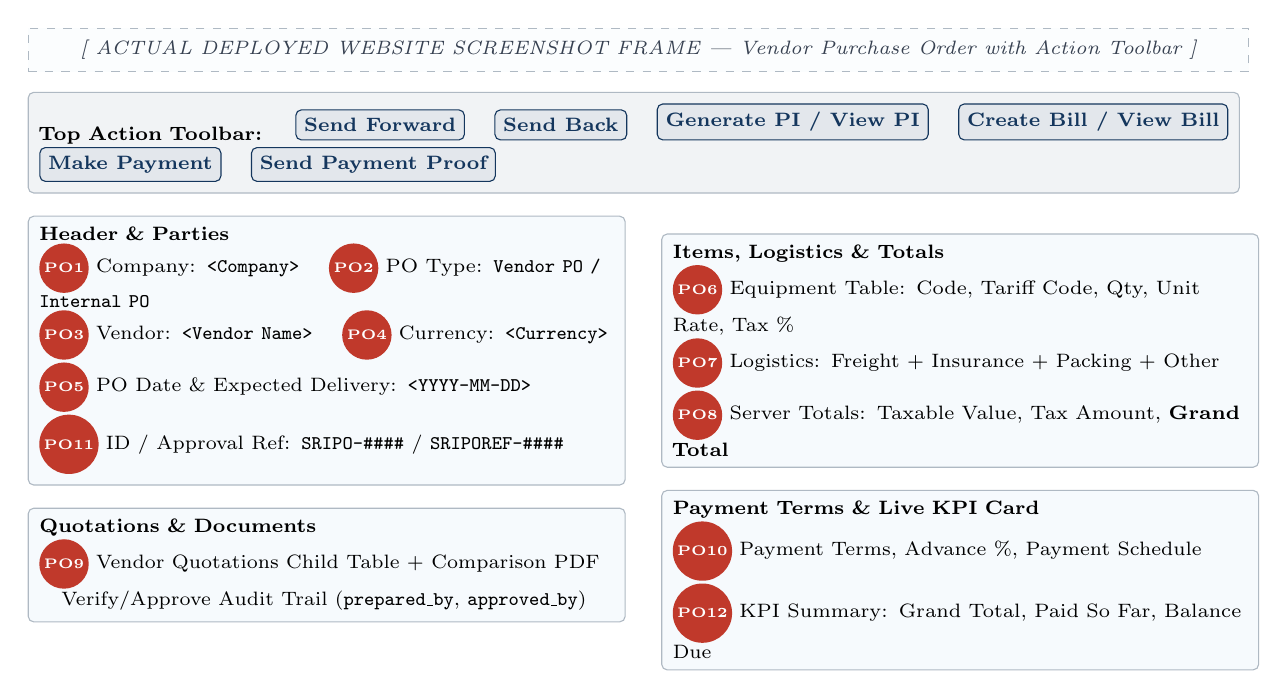
\begin{tikzpicture}[node distance=0.32cm and 0.4cm]
    \node[draw=bordergray, dashed, fill=softblue!20, minimum width=15.5cm, minimum height=0.55cm, font=\scriptsize\itshape, text=darkgray] (pobanner) at (0,0)
        {[ ACTUAL DEPLOYED WEBSITE SCREENSHOT FRAME --- Vendor Purchase Order with Action Toolbar ]};

    % Toolbar
    \node[uibox, fill=navyblue!6, text width=15.1cm, below=0.25cm of pobanner.south west, anchor=north west] (potbar) {
        \textbf{Top Action Toolbar:} \quad
        \tikz\node[uibtn]{Send Forward}; \quad
        \tikz\node[uibtn]{Send Back}; \quad
        \tikz\node[uibtn]{Generate PI / View PI}; \quad
        \tikz\node[uibtn]{Create Bill / View Bill}; \quad
        \tikz\node[uibtn]{Make Payment}; \quad
        \tikz\node[uibtn]{Send Payment Proof};
    };

    % Grid left & right
    \node[uibox, text width=7.3cm, below=0.28cm of potbar.south west, anchor=north west] (posec1) {
        \textbf{Header \& Parties}\\
        \pin{PO1} Company: \texttt{<Company>} \quad \pin{PO2} PO Type: \texttt{Vendor PO / Internal PO}\\
        \pin{PO3} Vendor: \texttt{<Vendor Name>} \quad \pin{PO4} Currency: \texttt{<Currency>}\\
        \pin{PO5} PO Date \& Expected Delivery: \texttt{<YYYY-MM-DD>}\\
        \pin{PO11} ID / Approval Ref: \texttt{SRIPO-\#\#\#\#} / \texttt{SRIPOREF-\#\#\#\#}
    };
    \node[uibox, text width=7.3cm, right=0.45cm of posec1] (posec2) {
        \textbf{Items, Logistics \& Totals}\\
        \pin{PO6} Equipment Table: Code, Tariff Code, Qty, Unit Rate, Tax \%\\
        \pin{PO7} Logistics: Freight + Insurance + Packing + Other\\
        \pin{PO8} Server Totals: Taxable Value, Tax Amount, \textbf{Grand Total}
    };
    \node[uibox, text width=7.3cm, below=0.28cm of posec1] (posec3) {
        \textbf{Quotations \& Documents}\\
        \pin{PO9} Vendor Quotations Child Table + Comparison PDF\\
        \quad Verify/Approve Audit Trail (\texttt{prepared\_by}, \texttt{approved\_by})
    };
    \node[uibox, text width=7.3cm, below=0.28cm of posec2] (posec4) {
        \textbf{Payment Terms \& Live KPI Card}\\
        \pin{PO10} Payment Terms, Advance \%, Payment Schedule\\
        \pin{PO12} KPI Summary: Grand Total, Paid So Far, Balance Due
    };
\end{tikzpicture}}
\end{webframe}

\begin{figure}[htbp]
    \centering
    \resizebox{\textwidth}{!}{%
    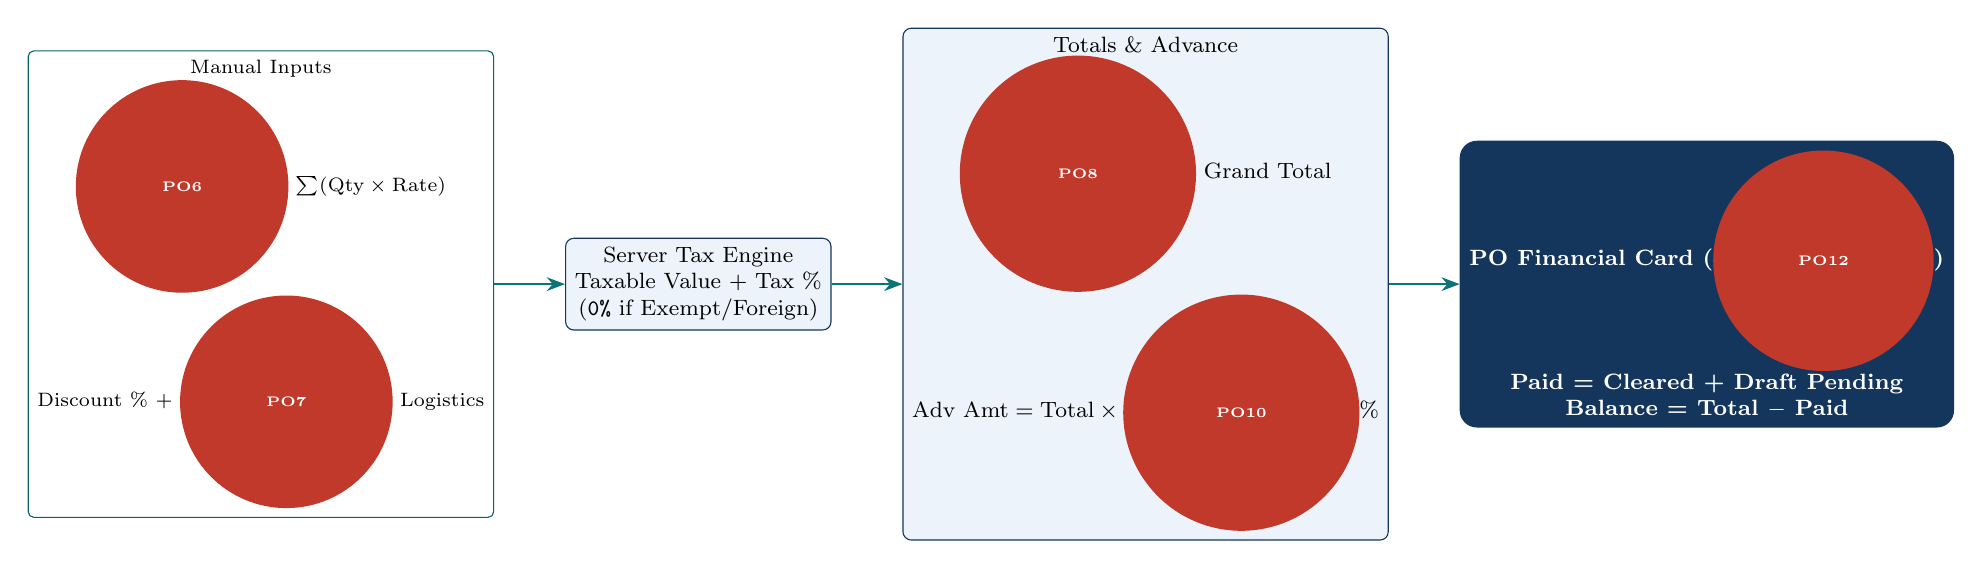
\begin{tikzpicture}[node distance=0.7cm and 0.9cm]
        \node (inp) [datanode] {Manual Inputs\\\pin{PO6} $\sum(\text{Qty} \times \text{Rate})$\\Discount \% + \pin{PO7} Logistics};
        \node (tax) [process, right=of inp] {Server Tax Engine\\Taxable Value + Tax \%\\(\texttt{0\%} if Exempt/Foreign)};
        \node (tot) [process, right=of tax] {Totals \& Advance\\\pin{PO8} Grand Total\\$\text{Adv Amt} = \text{Total} \times \pin{PO10}\%$};
        \node (kpi) [startstop, right=of tot] {PO Financial Card (\pin{PO12})\\Paid = Cleared + Draft Pending\\Balance = Total $-$ Paid};

        \draw [dataarrow] (inp) -- (tax);
        \draw [dataarrow] (tax) -- (tot);
        \draw [dataarrow] (tot) -- (kpi);
    \end{tikzpicture}}
    \caption{Vendor Purchase Order Server Calculation \& Financial KPI Dataflow}
    \label{fig:po-dataflow}
\end{figure}

\begin{rulebox}{Yearwise \& Monthwise Reporting}
In \textbf{Vendor Purchase Order List}, click \textbf{PO Amount Summary} to slice totals, statuses, and vendor rankings by \textbf{Year}, \textbf{Month}, or custom date range.
\end{rulebox}

% -------------------------------------------------------------------------
% CHAPTER 6: PROFORMA INVOICE
% -------------------------------------------------------------------------
\chapter{Preparing a Proforma Invoice (PI)}
\index{Proforma Invoice!Creation}\index{Proforma Invoice!Margin Rule}

\section{Proforma Invoice Generation \& Validation Flowchart}

\begin{figure}[htbp]
    \centering
    \resizebox{\textwidth}{!}{%
    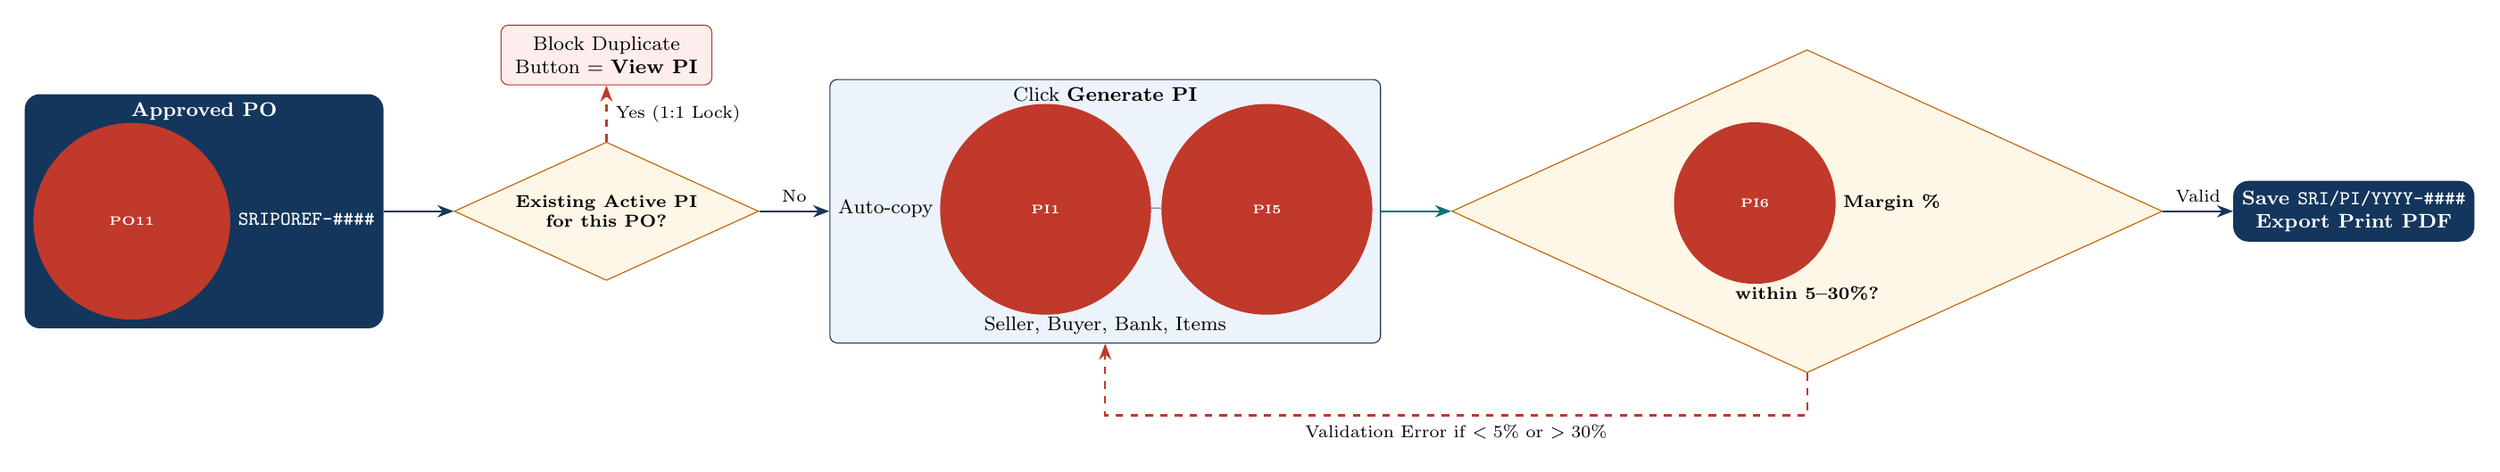
\begin{tikzpicture}[node distance=0.8cm and 1.0cm]
        \node (poa) [startstop] {Approved PO\\\pin{PO11} \texttt{SRIPOREF-\#\#\#\#}};
        \node (chk) [decision, right=of poa] {Existing Active PI\\for this PO?};
        \node (blk) [process, above=0.8cm of chk, draw=pinred, fill=softred] {Block Duplicate\\Button = \textbf{View PI}};
        \node (gen) [process, right=of chk] {Click \textbf{Generate PI}\\Auto-copy \pin{PI1}--\pin{PI5}\\Seller, Buyer, Bank, Items};
        \node (mrg) [decision, right=of gen] {\pin{PI6} Margin \%\\within 5--30\%?};
        \node (save) [startstop, right=of mrg] {Save \texttt{SRI/PI/YYYY-\#\#\#\#}\\Export Print PDF};

        \draw [arrow] (poa) -- (chk);
        \draw [backarrow] (chk) -- node[right, font=\scriptsize]{Yes (1:1 Lock)} (blk);
        \draw [arrow] (chk) -- node[above, font=\scriptsize]{No} (gen);
        \draw [dataarrow] (gen) -- (mrg);
        \draw [backarrow] (mrg.south) -- ++(0,-0.6) -| node[pos=0.25, below, font=\scriptsize]{Validation Error if $<5\%$ or $>30\%$} (gen.south);
        \draw [arrow] (mrg) -- node[above, font=\scriptsize]{Valid} (save);
    \end{tikzpicture}}
    \caption{Proforma Invoice Creation, 1-to-1 Lock, and Margin Gate Flowchart}
    \label{fig:pi-workflow}
\end{figure}

\section{Website Screenshot Layout \& Marked Fields (\texttt{Proforma Invoice})}

\begin{webframe}{proforma-invoice/SRI-PI-YYYY-XXXX}{Actual Website Screen: Proforma Invoice Form}
\centering
\resizebox{0.97\textwidth}{!}{%
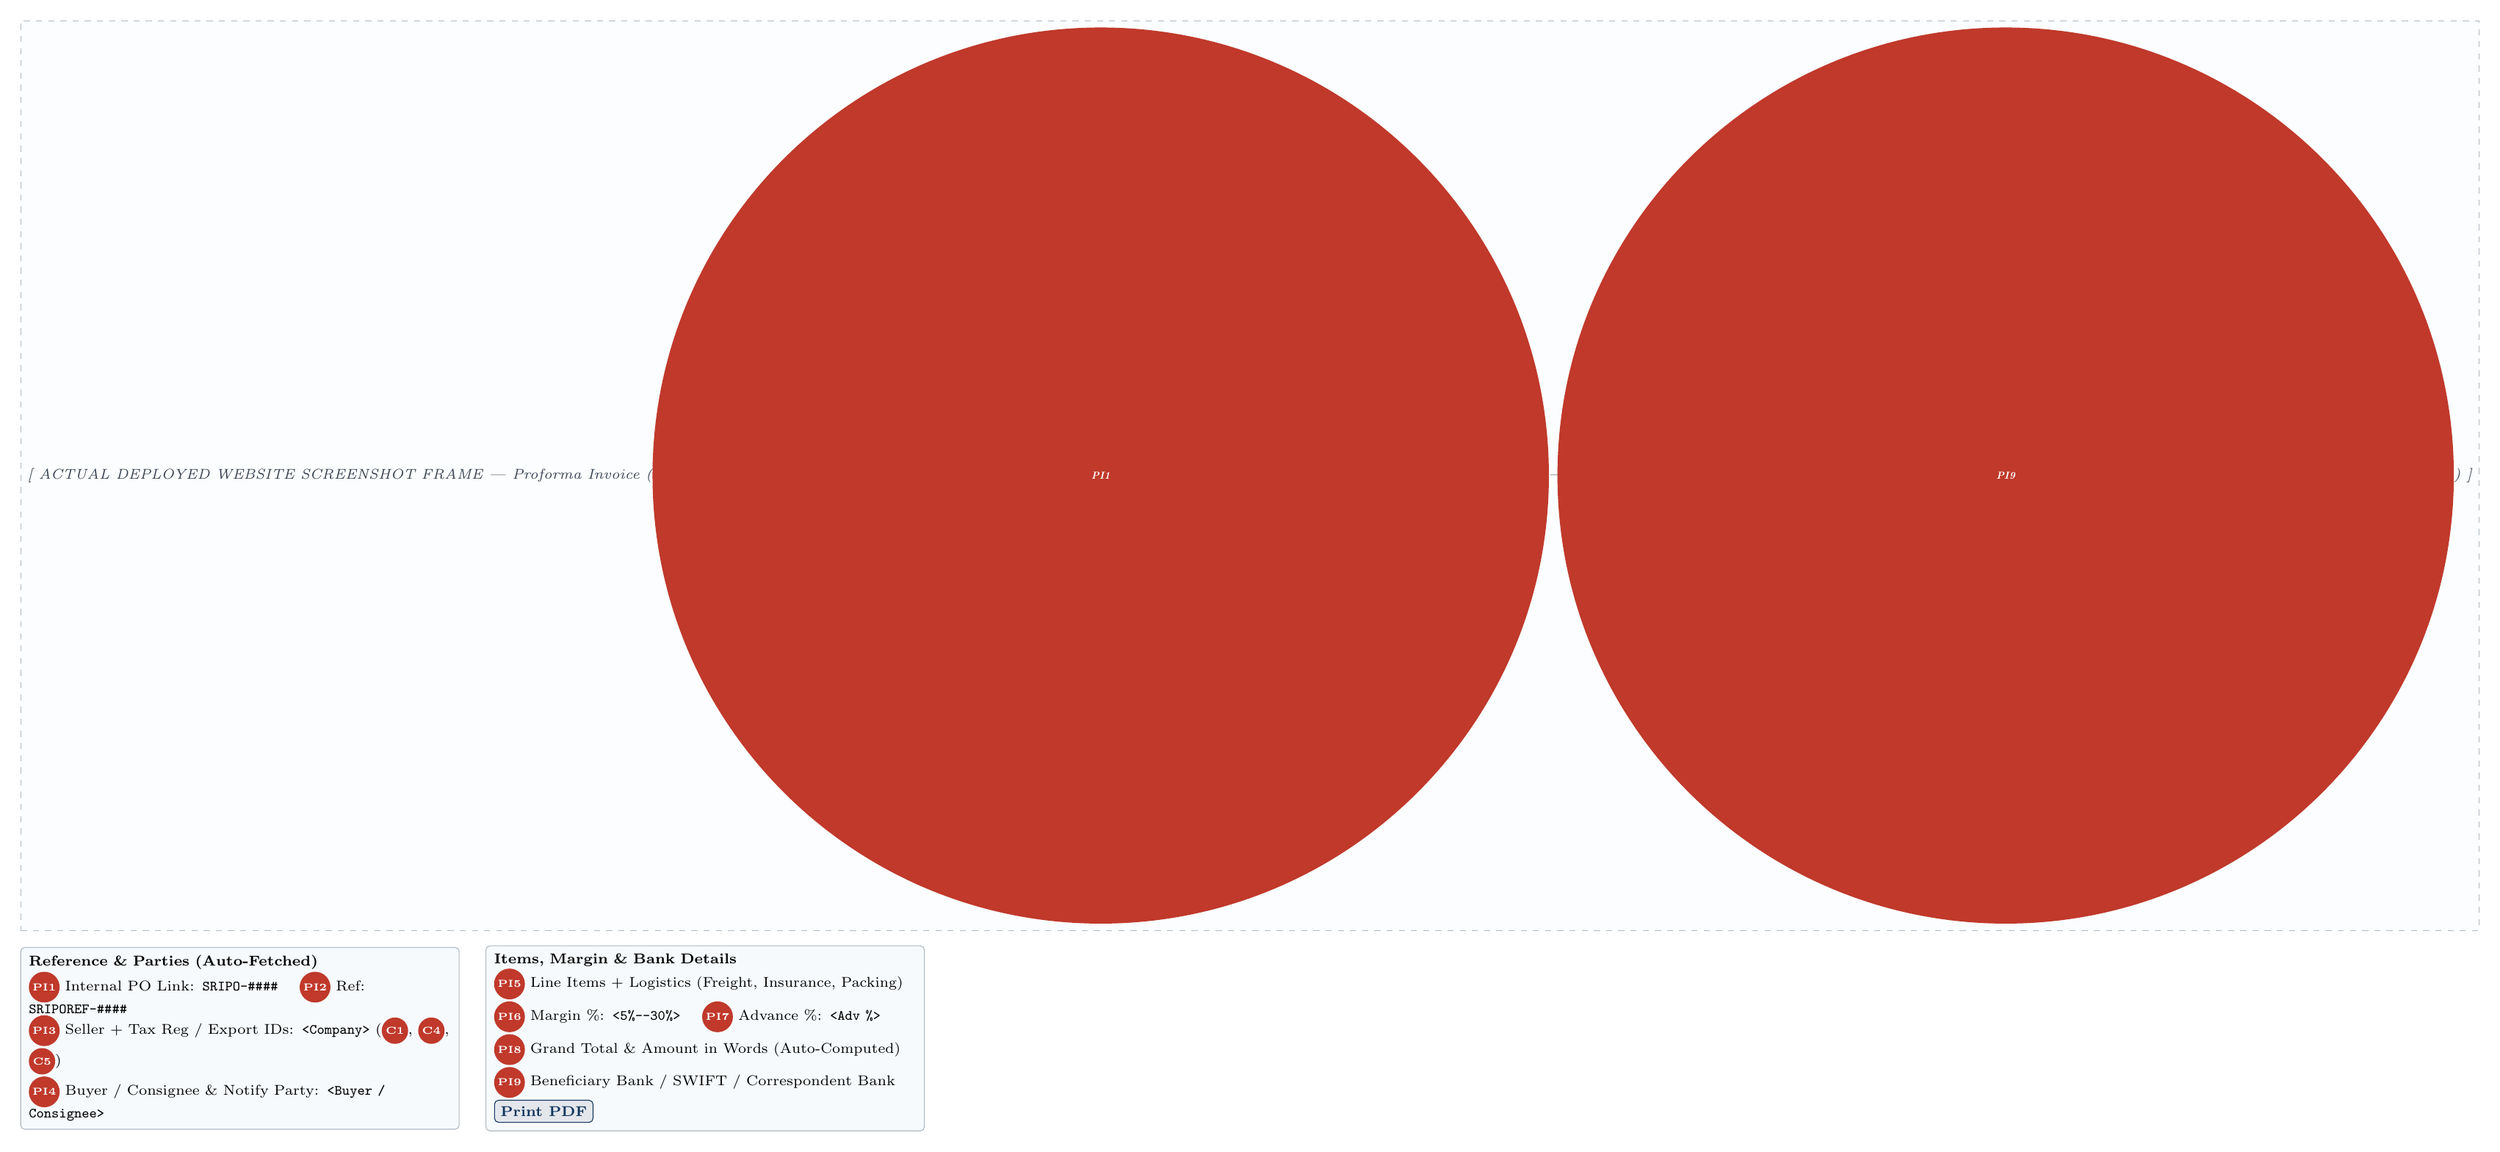
\begin{tikzpicture}[node distance=0.32cm and 0.45cm]
    \node[draw=bordergray, dashed, fill=softblue!20, minimum width=15.5cm, minimum height=0.55cm, font=\scriptsize\itshape, text=darkgray] (pibanner) at (0,0)
        {[ ACTUAL DEPLOYED WEBSITE SCREENSHOT FRAME --- Proforma Invoice (\pin{PI1}--\pin{PI9}) ]};

    \node[uibox, text width=7.3cm, below=0.28cm of pibanner.south west, anchor=north west] (pisec1) {
        \textbf{Reference \& Parties (Auto-Fetched)}\\
        \pin{PI1} Internal PO Link: \texttt{SRIPO-\#\#\#\#} \quad \pin{PI2} Ref: \texttt{SRIPOREF-\#\#\#\#}\\
        \pin{PI3} Seller + Tax Reg / Export IDs: \texttt{<Company>} (\pin{C1}, \pin{C4}, \pin{C5})\\
        \pin{PI4} Buyer / Consignee \& Notify Party: \texttt{<Buyer / Consignee>}
    };
    \node[uibox, text width=7.3cm, right=0.45cm of pisec1] (pisec2) {
        \textbf{Items, Margin \& Bank Details}\\
        \pin{PI5} Line Items + Logistics (Freight, Insurance, Packing)\\
        \pin{PI6} Margin \%: \texttt{<5\%--30\%>} \quad \pin{PI7} Advance \%: \texttt{<Adv \%>}\\
        \pin{PI8} Grand Total \& Amount in Words (Auto-Computed)\\
        \pin{PI9} Beneficiary Bank / SWIFT / Correspondent Bank \hfill \tikz\node[uibtn]{Print PDF};
    };
\end{tikzpicture}}
\end{webframe}

% -------------------------------------------------------------------------
% CHAPTER 7: PURCHASE INVOICE
% -------------------------------------------------------------------------
\chapter{Preparing a Purchase Invoice (Vendor Bill)}
\index{Purchase Invoice!Creation}\index{Purchase Invoice!Milestone Mapping}\index{Payment Invoice|see{Purchase Invoice}}

\section{Purchase Invoice Creation \& GL Posting Flowchart}

\begin{figure}[htbp]
    \centering
    \resizebox{\textwidth}{!}{%
    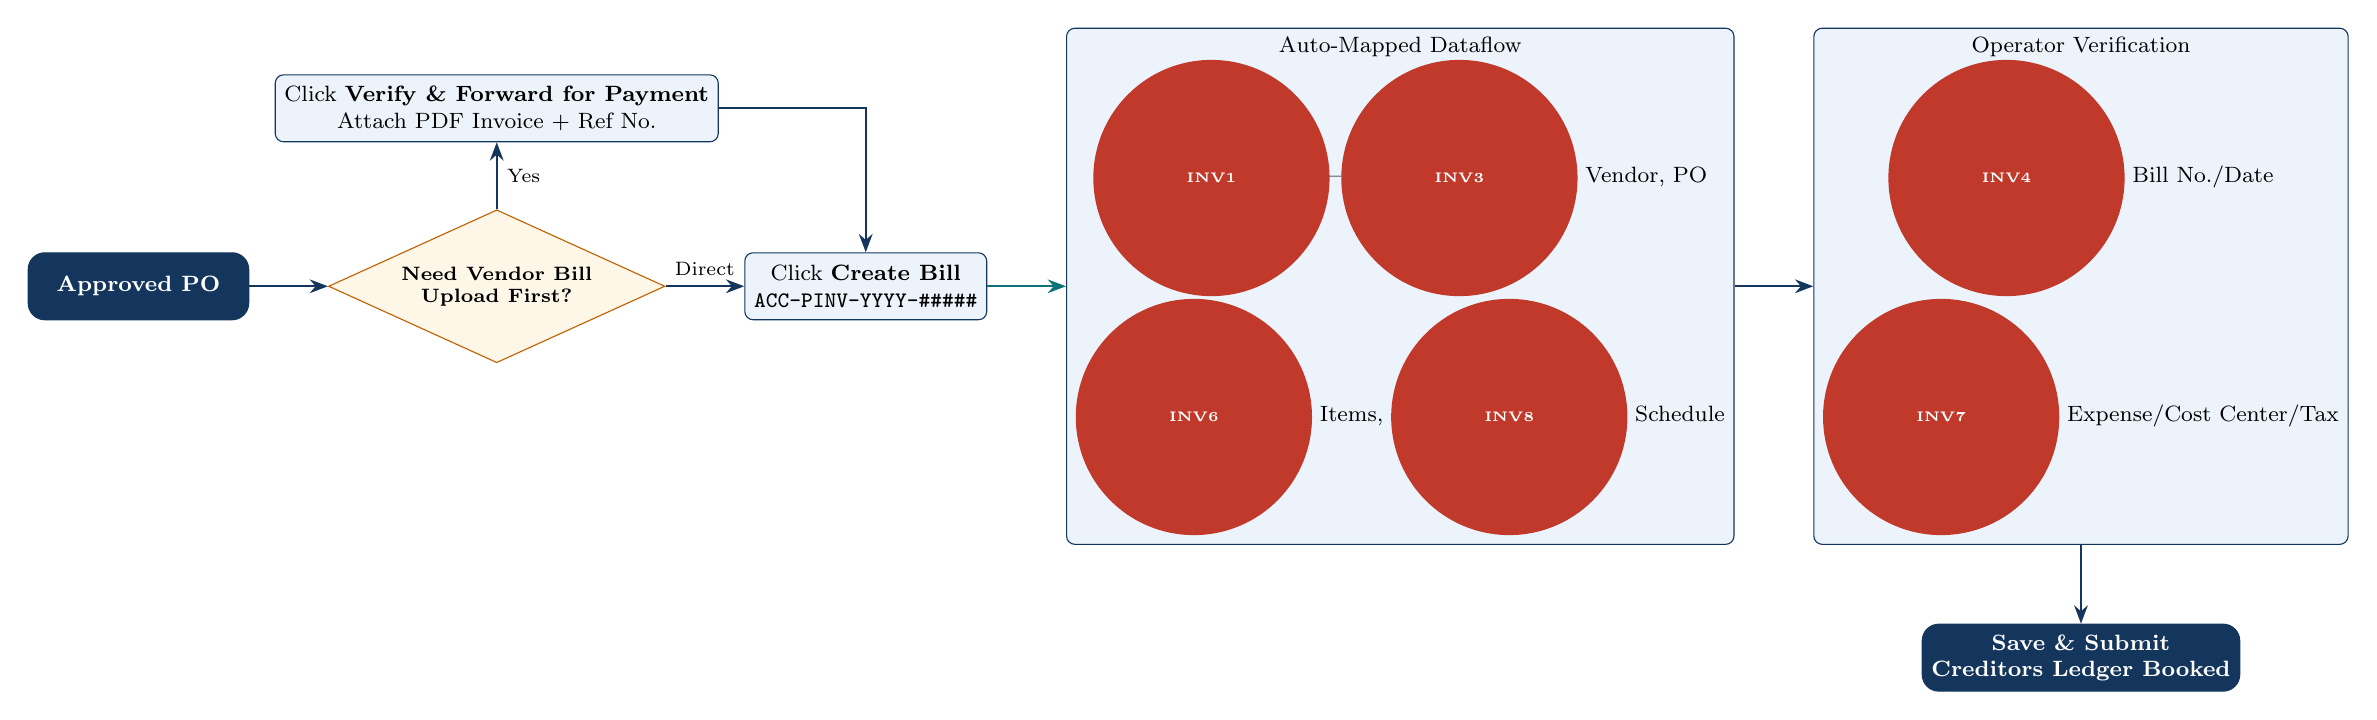
\begin{tikzpicture}[node distance=0.85cm and 1.0cm]
        \node (ap) [startstop] {Approved PO};
        \node (opt) [decision, right=of ap] {Need Vendor Bill\\Upload First?};
        \node (vfw) [process, above=0.85cm of opt] {Click \textbf{Verify \& Forward for Payment}\\Attach PDF Invoice + Ref No.};
        \node (cb) [process, right=of opt] {Click \textbf{Create Bill}\\\texttt{ACC-PINV-YYYY-\#\#\#\#\#}};
        \node (map) [process, right=of cb] {Auto-Mapped Dataflow\\\pin{INV1}--\pin{INV3} Vendor, PO\\\pin{INV6} Items, \pin{INV8} Schedule};
        \node (acc) [process, right=of map] {Operator Verification\\\pin{INV4} Bill No./Date\\\pin{INV7} Expense/Cost Center/Tax};
        \node (sub) [startstop, below=1.0cm of acc] {Save \& \textbf{Submit}\\Creditors Ledger Booked};

        \draw [arrow] (ap) -- (opt);
        \draw [arrow] (opt) -- node[right, font=\scriptsize]{Yes} (vfw);
        \draw [arrow] (vfw) -| (cb);
        \draw [arrow] (opt) -- node[above, font=\scriptsize]{Direct} (cb);
        \draw [dataarrow] (cb) -- (map);
        \draw [arrow] (map) -- (acc);
        \draw [arrow] (acc) -- (sub);
    \end{tikzpicture}}
    \caption{Vendor Bill Forwarding, Field Transfer, and General Ledger Posting Flow}
    \label{fig:pinv-flow}
\end{figure}

\section{Website Screenshot Layout \& Marked Fields (\texttt{Purchase Invoice})}

\begin{webframe}{purchase-invoice/ACC-PINV-YYYY-XXXXX}{Actual Website Screen: Purchase Invoice Form}
\centering
\resizebox{0.97\textwidth}{!}{%
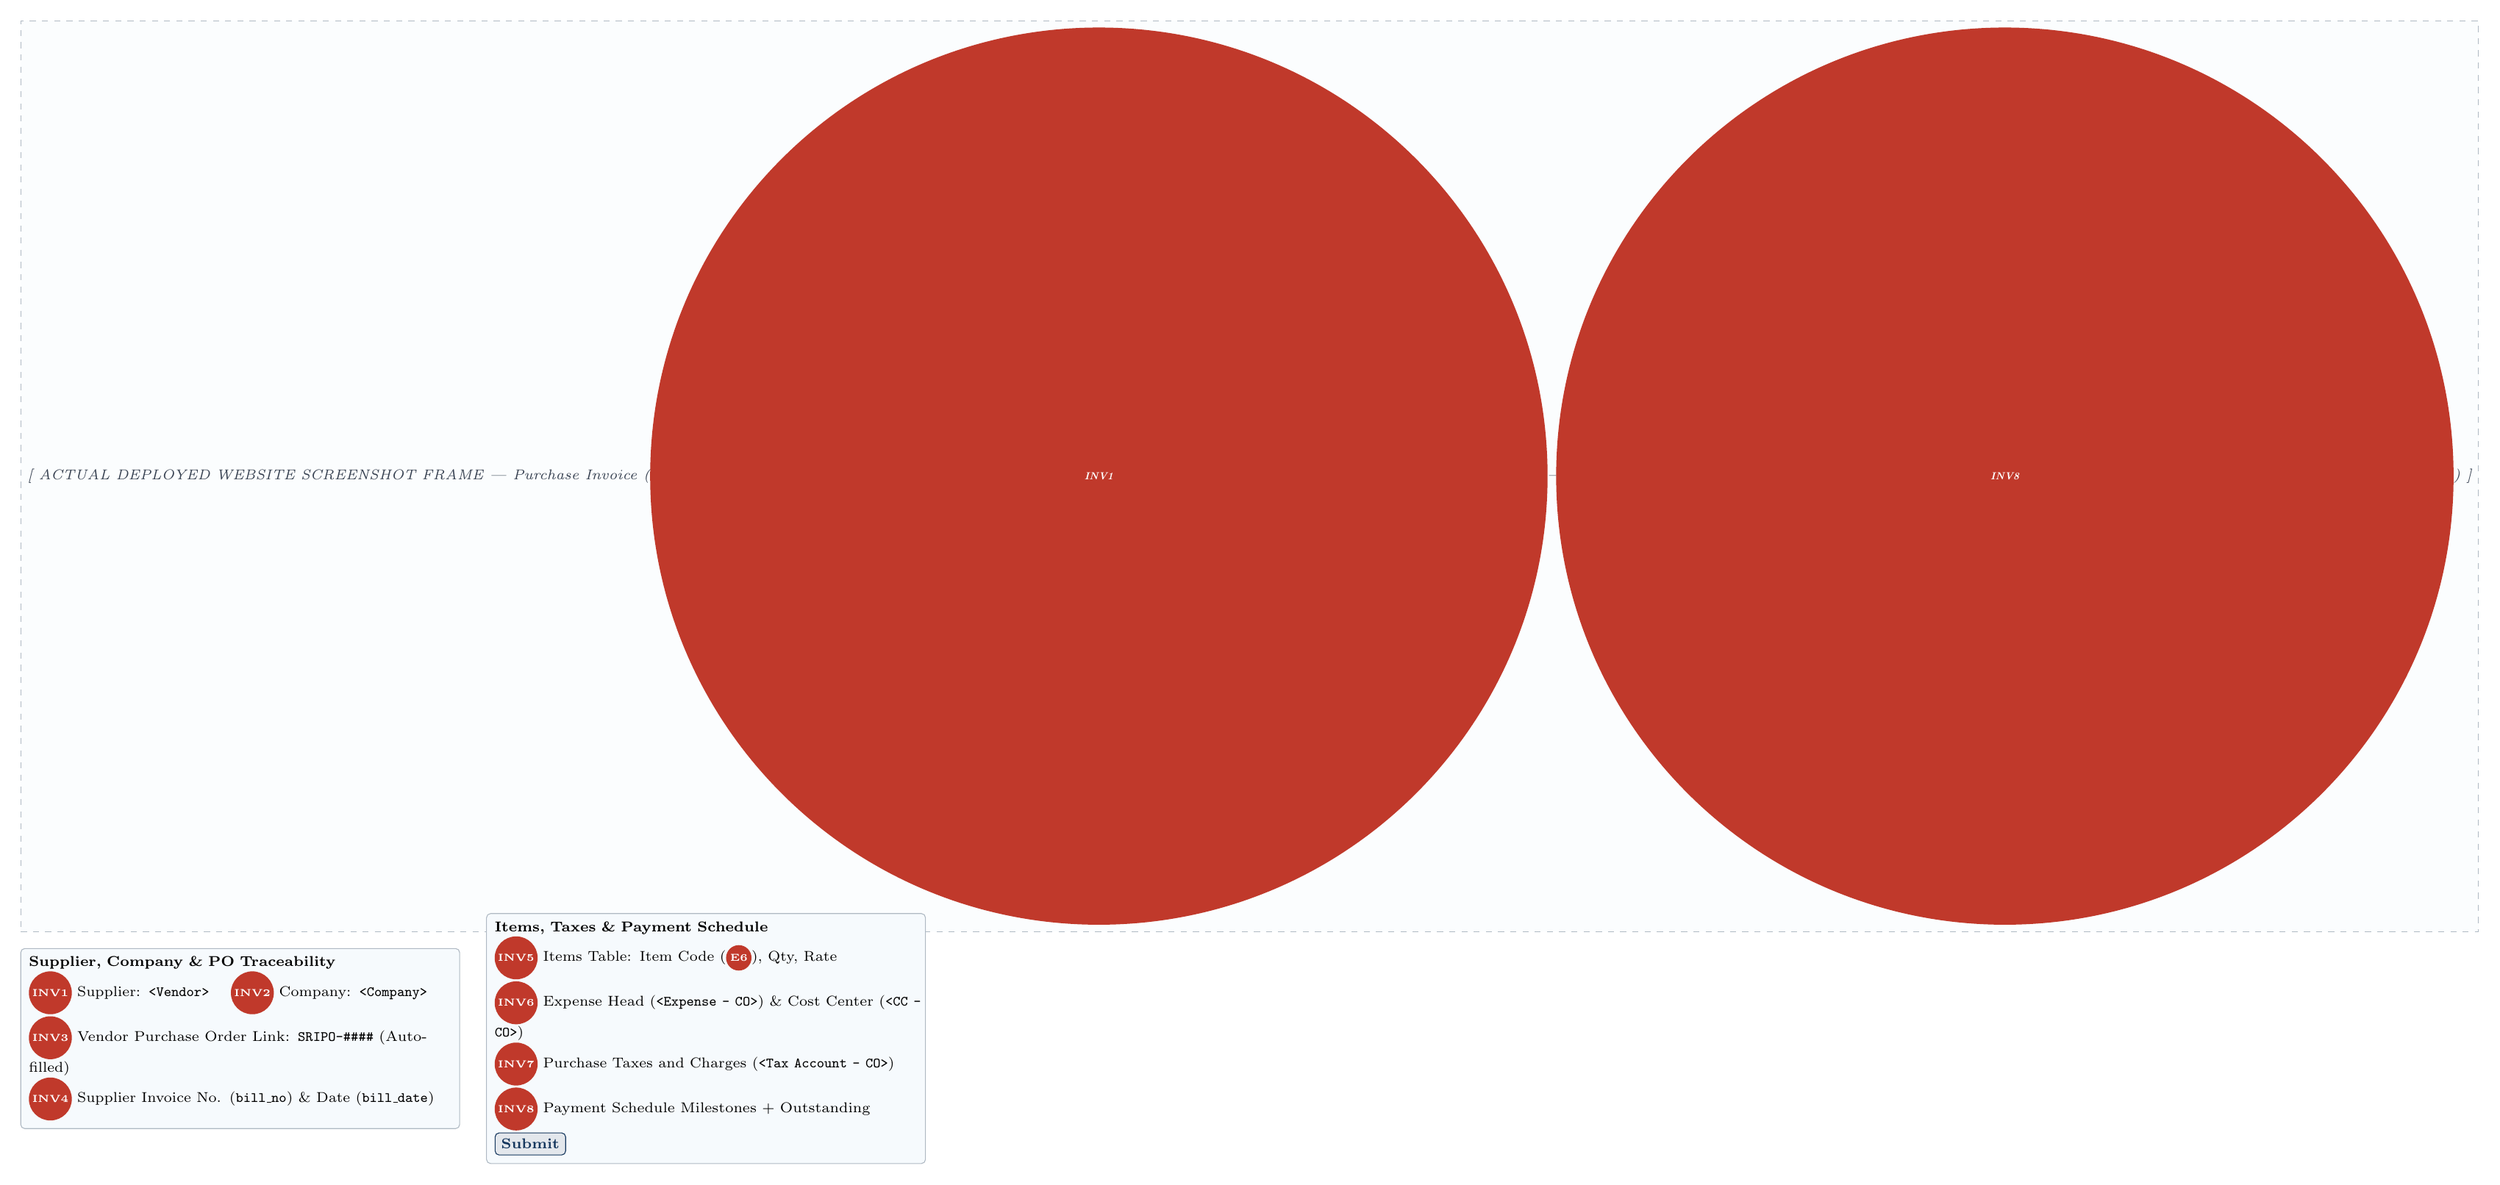
\begin{tikzpicture}[node distance=0.32cm and 0.45cm]
    \node[draw=bordergray, dashed, fill=softblue!20, minimum width=15.5cm, minimum height=0.55cm, font=\scriptsize\itshape, text=darkgray] (invbanner) at (0,0)
        {[ ACTUAL DEPLOYED WEBSITE SCREENSHOT FRAME --- Purchase Invoice (\pin{INV1}--\pin{INV8}) ]};

    \node[uibox, text width=7.3cm, below=0.28cm of invbanner.south west, anchor=north west] (invsec1) {
        \textbf{Supplier, Company \& PO Traceability}\\
        \pin{INV1} Supplier: \texttt{<Vendor>} \quad \pin{INV2} Company: \texttt{<Company>}\\
        \pin{INV3} Vendor Purchase Order Link: \texttt{SRIPO-\#\#\#\#} (Auto-filled)\\
        \pin{INV4} Supplier Invoice No. (\texttt{bill\_no}) \& Date (\texttt{bill\_date})
    };
    \node[uibox, text width=7.3cm, right=0.45cm of invsec1] (invsec2) {
        \textbf{Items, Taxes \& Payment Schedule}\\
        \pin{INV5} Items Table: Item Code (\pin{E6}), Qty, Rate\\
        \pin{INV6} Expense Head (\texttt{<Expense - CO>}) \& Cost Center (\texttt{<CC - CO>})\\
        \pin{INV7} Purchase Taxes and Charges (\texttt{<Tax Account - CO>})\\
        \pin{INV8} Payment Schedule Milestones + Outstanding \hfill \tikz\node[uibtn]{Submit};
    };
\end{tikzpicture}}
\end{webframe}

% -------------------------------------------------------------------------
% CHAPTER 8: PAYMENT ENTRIES & RECONCILIATION
% -------------------------------------------------------------------------
\chapter{Preparing Payment Entries \& Advance Reconciliation}
\index{Payment Entry!Creation}\index{Payment Entry!Draft Pending Reconciliation}\index{Make Payment Dialog}

\section{Dual-Path Payment Entry \& Approval Flowchart}

\begin{figure}[htbp]
    \centering
    \resizebox{\textwidth}{!}{%
    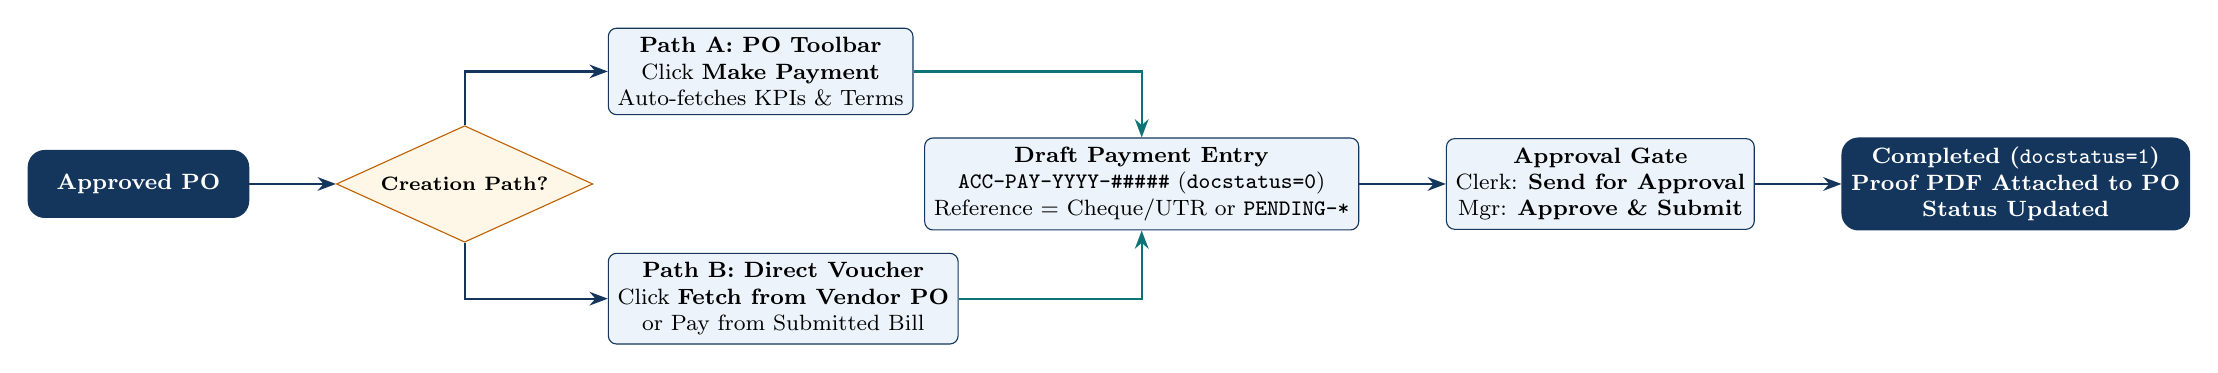
\begin{tikzpicture}[node distance=0.85cm and 1.1cm]
        \node (po) [startstop] {Approved PO};
        \node (mth) [decision, right=of po] {Creation Path?};
        \node (dlg) [process, above right=0.5cm and 1.0cm of mth] {\textbf{Path A: PO Toolbar}\\Click \textbf{Make Payment}\\Auto-fetches KPIs \& Terms};
        \node (fet) [process, below right=0.5cm and 1.0cm of mth] {\textbf{Path B: Direct Voucher}\\Click \textbf{Fetch from Vendor PO}\\or Pay from Submitted Bill};

        \node (dft) [process, right=4.2cm of mth] {\textbf{Draft Payment Entry}\\\texttt{ACC-PAY-YYYY-\#\#\#\#\#} (\texttt{docstatus=0})\\Reference = Cheque/UTR or \texttt{PENDING-*}};
        \node (apv) [process, right=of dft] {\textbf{Approval Gate}\\Clerk: \textbf{Send for Approval}\\Mgr: \textbf{Approve \& Submit}};
        \node (cmp) [startstop, right=of apv] {\textbf{Completed (\texttt{docstatus=1})}\\Proof PDF Attached to PO\\Status Updated};

        \draw [arrow] (po) -- (mth);
        \draw [arrow] (mth) |- (dlg);
        \draw [arrow] (mth) |- (fet);
        \draw [dataarrow] (dlg) -| (dft);
        \draw [dataarrow] (fet) -| (dft);
        \draw [arrow] (dft) -- (apv);
        \draw [arrow] (apv) -- (cmp);
    \end{tikzpicture}}
    \caption{Payment Entry Creation, Draft Pending Tracking, and Approval Settlement Flow}
    \label{fig:payment-workflow}
\end{figure}

\section{Live Pending Balance \& Advance Reconciliation Dataflow}

\begin{figure}[htbp]
    \centering
    \resizebox{\textwidth}{!}{%
    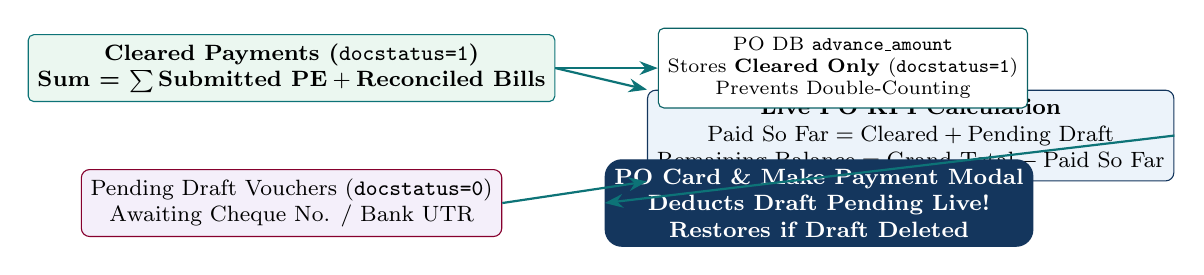
\begin{tikzpicture}[node distance=0.75cm and 1.0cm]
        \node (clr) [rolebox] {Cleared Payments (\texttt{docstatus=1})\\Sum = $\sum \text{Submitted PE} + \text{Reconciled Bills}$};
        \node (pen) [docnode, below=0.85cm of clr] {Pending Draft Vouchers (\texttt{docstatus=0})\\Awaiting Cheque No. / Bank UTR};
        \node (sum) [process, right=1.5cm of $(clr.east)!0.5!(pen.east)$] {\textbf{Live PO KPI Calculation}\\$\text{Paid So Far} = \text{Cleared} + \text{Pending Draft}$\\$\text{Remaining Balance} = \text{Grand Total} - \text{Paid So Far}$};
        \node (db) [datanode, right=1.3cm of clr] {PO DB \texttt{advance\_amount}\\Stores \textbf{Cleared Only} (\texttt{docstatus=1})\\Prevents Double-Counting};
        \node (ui) [startstop, right=1.3cm of pen] {PO Card \& Make Payment Modal\\Deducts Draft Pending Live!\\Restores if Draft Deleted};

        \draw [dataarrow] (clr.east) -- (sum.north west);
        \draw [dataarrow] (pen.east) -- (sum.south west);
        \draw [dataarrow] (clr.east) -- (db.west);
        \draw [dataarrow] (sum.east) -- (ui.west);
    \end{tikzpicture}}
    \caption{Live Balance Formula: Pending Draft Deduction vs.\ Cleared Ledger Persistence}
    \label{fig:payment-balance-dataflow}
\end{figure}

\section{Website Screenshot Layout \& Marked Fields (\texttt{Payment Entry})}

\begin{webframe}{payment-entry/ACC-PAY-YYYY-XXXXX}{Actual Website Screen: Payment Entry \& Make Payment Modal}
\centering
\resizebox{0.97\textwidth}{!}{%
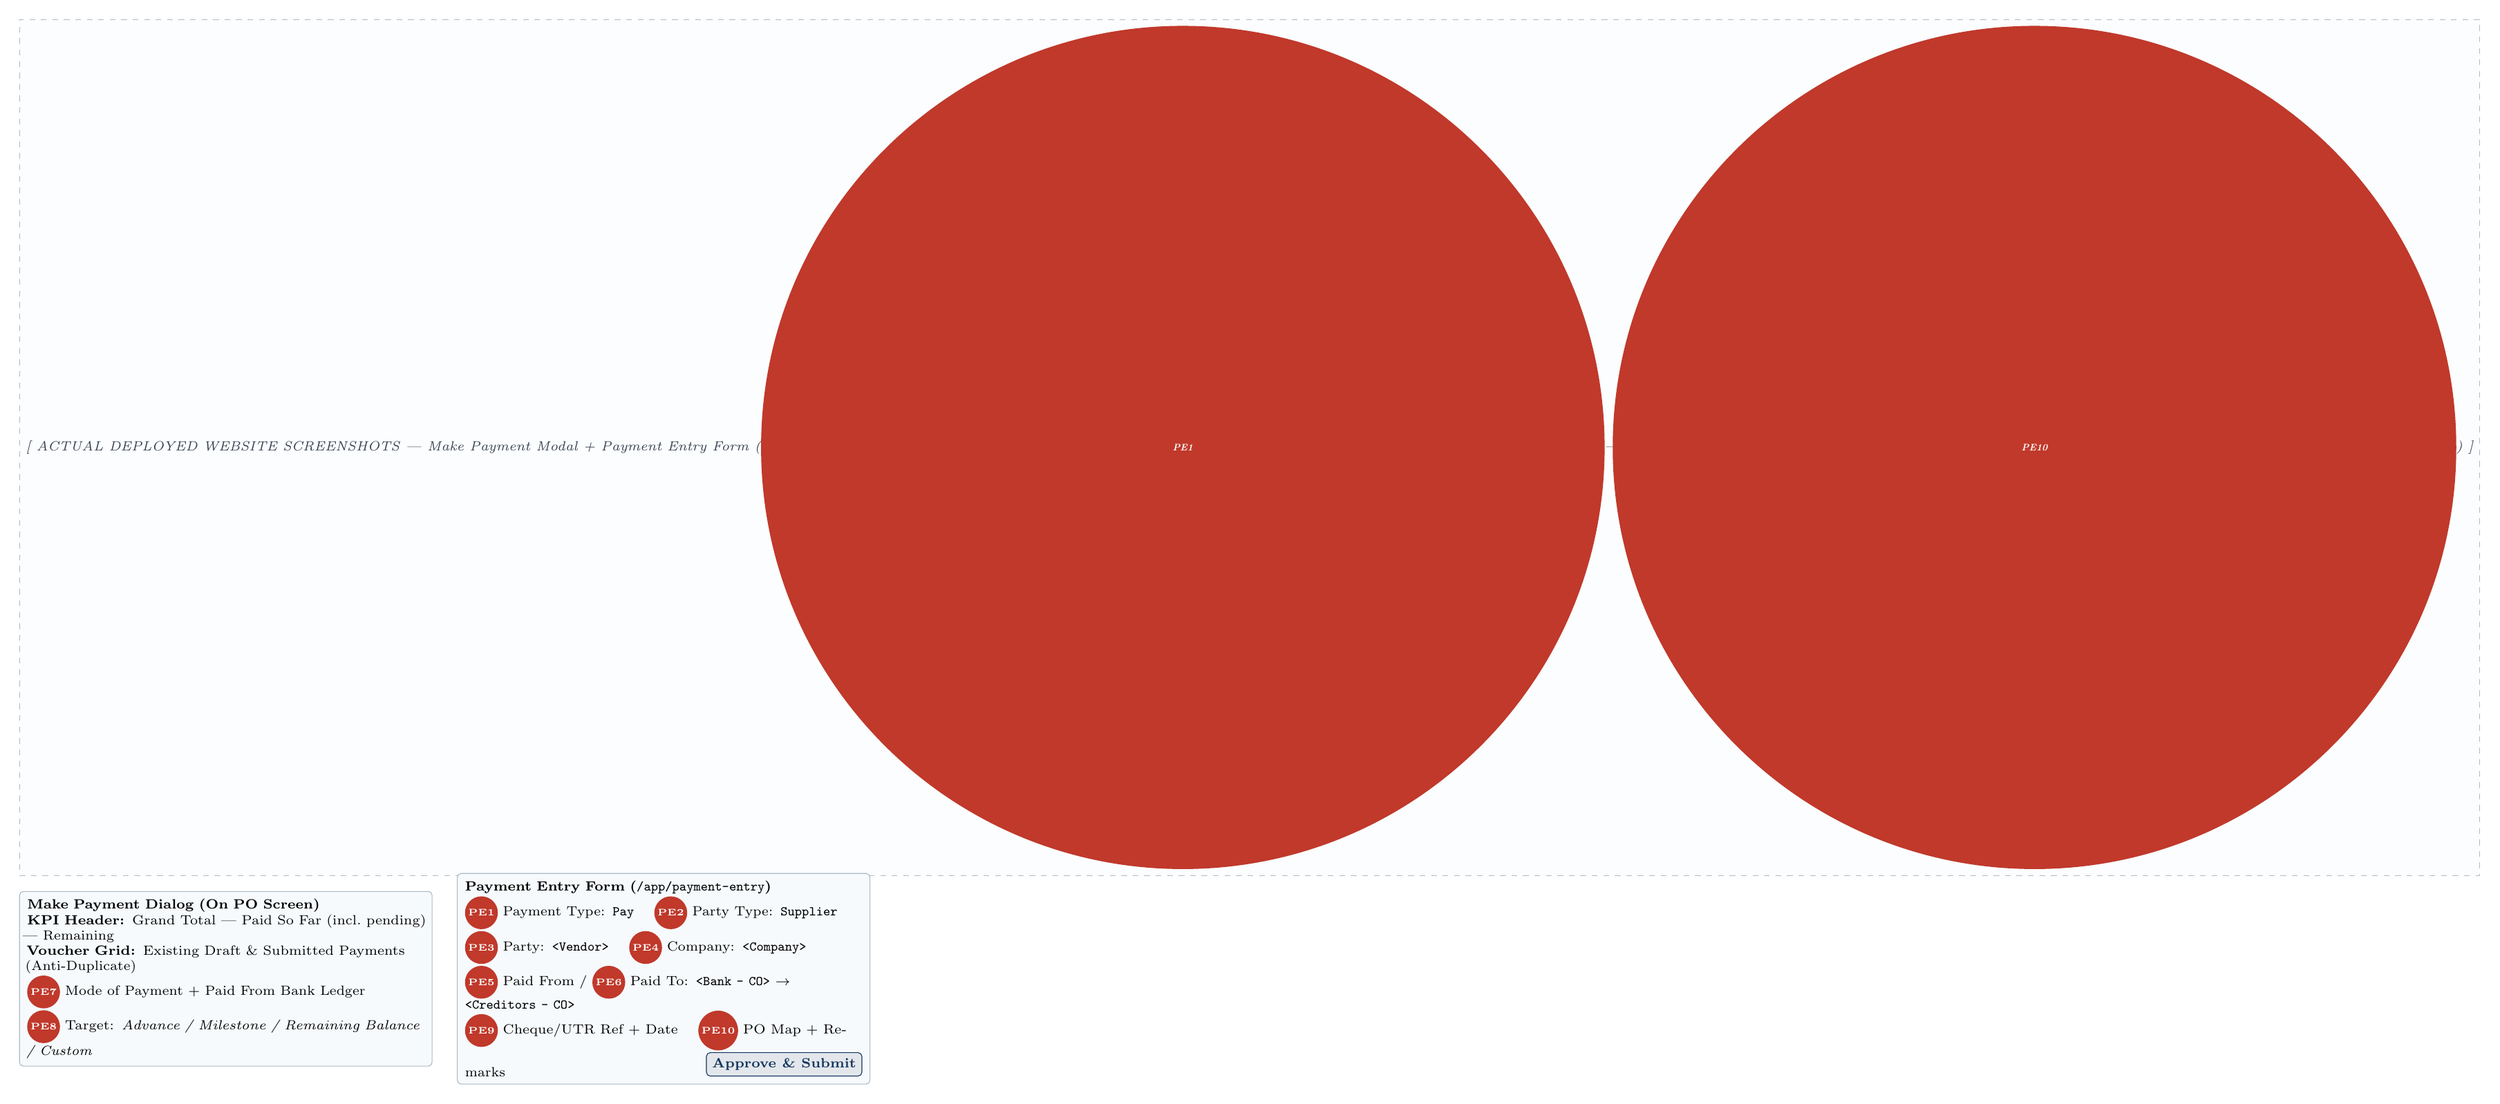
\begin{tikzpicture}[node distance=0.32cm and 0.45cm]
    \node[draw=bordergray, dashed, fill=softblue!20, minimum width=15.5cm, minimum height=0.55cm, font=\scriptsize\itshape, text=darkgray] (pebanner) at (0,0)
        {[ ACTUAL DEPLOYED WEBSITE SCREENSHOTS --- Make Payment Modal + Payment Entry Form (\pin{PE1}--\pin{PE10}) ]};

    \node[uibox, text width=7.3cm, below=0.28cm of pebanner.south west, anchor=north west] (pesec1) {
        \textbf{Make Payment Dialog (On PO Screen)}\\
        \textbf{KPI Header:} Grand Total | Paid So Far (incl.\ pending) | Remaining\\
        \textbf{Voucher Grid:} Existing Draft \& Submitted Payments (Anti-Duplicate)\\
        \pin{PE7} Mode of Payment + Paid From Bank Ledger\\
        \pin{PE8} Target: \textit{Advance / Milestone / Remaining Balance / Custom}
    };
    \node[uibox, text width=7.3cm, right=0.45cm of pesec1] (pesec2) {
        \textbf{Payment Entry Form (\texttt{/app/payment-entry})}\\
        \pin{PE1} Payment Type: \texttt{Pay} \quad \pin{PE2} Party Type: \texttt{Supplier}\\
        \pin{PE3} Party: \texttt{<Vendor>} \quad \pin{PE4} Company: \texttt{<Company>}\\
        \pin{PE5} Paid From / \pin{PE6} Paid To: \texttt{<Bank - CO>} $\rightarrow$ \texttt{<Creditors - CO>}\\
        \pin{PE9} Cheque/UTR Ref + Date \quad \pin{PE10} PO Map + Remarks \hfill \tikz\node[uibtn]{Approve \& Submit};
    };
\end{tikzpicture}}
\end{webframe}

\begin{exercisebox}{Execute Full Payment Settlement Sequence}
\begin{enumerate}[leftmargin=1.5em, itemsep=1pt]
    \item On an Approved PO, click \textbf{Make Payment} and verify \pin{PE8} reflects \texttt{Remaining Balance = Grand Total - (Cleared + Draft Pending)}.
    \item Open an existing \texttt{Draft} Advance voucher, replace placeholder reference \pin{PE9} with real \texttt{<Cheque / Bank UTR>}, click \textbf{Save} $\rightarrow$ \textbf{Send for Approval} $\rightarrow$ \textbf{Approve \& Submit}.
    \item Confirm generated \texttt{Payment\_Proof\_ACC-PAY-YYYY-\#\#\#\#\#.pdf} attaches to the PO and status transitions to \texttt{Advance Paid} / \texttt{Partially Paid} / \texttt{Fully Paid}.
\end{enumerate}
\end{exercisebox}

% -------------------------------------------------------------------------
% CHAPTER 9: TROUBLESHOOTING DECISION FLOW & TABLE
% -------------------------------------------------------------------------
\chapter{Troubleshooting \& Quick Reference}
\index{Troubleshooting}

\section{Diagnostic Decision Flowchart}

\begin{figure}[htbp]
    \centering
    \resizebox{\textwidth}{!}{%
    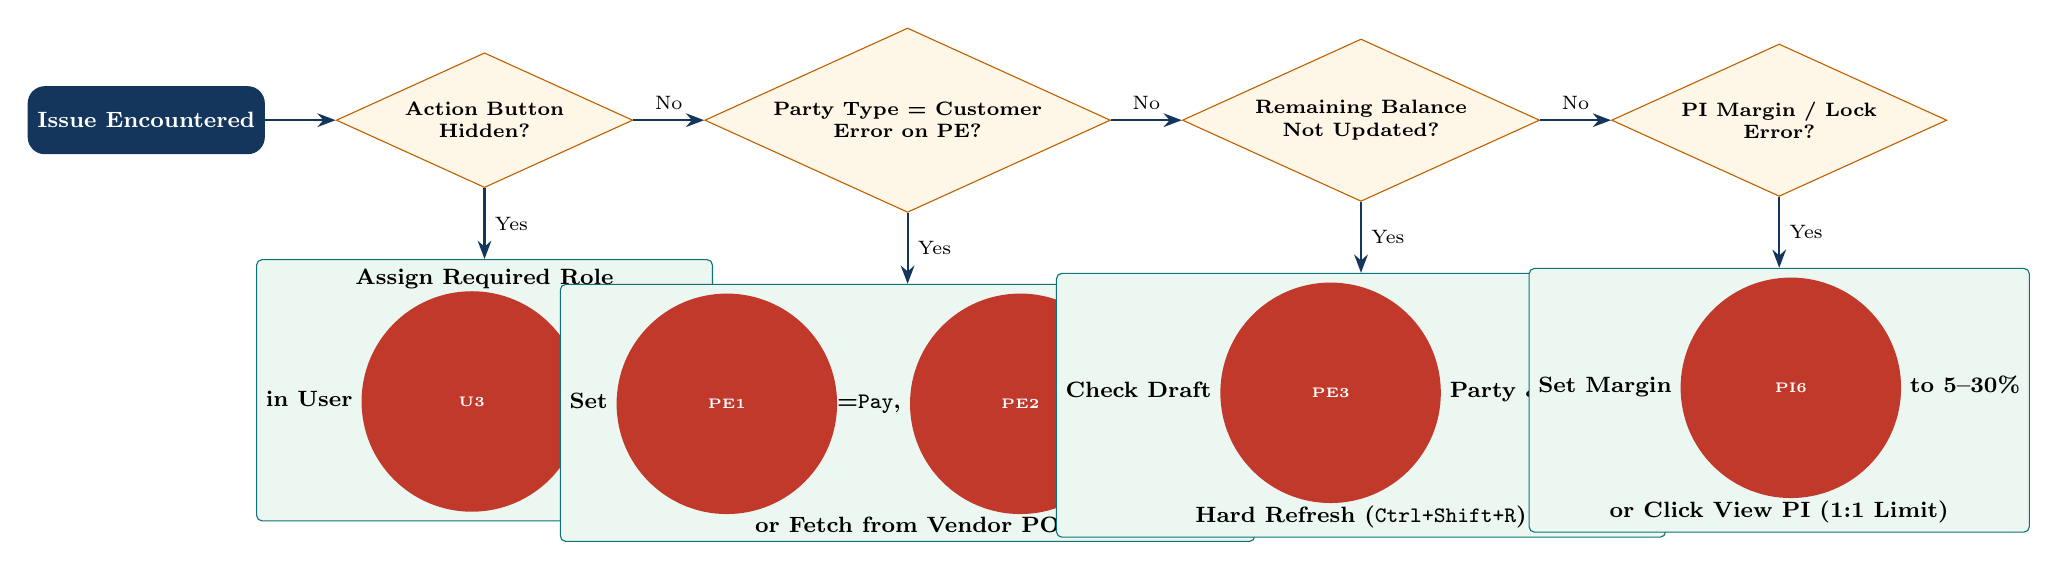
\begin{tikzpicture}[node distance=0.75cm and 0.9cm]
        \node (t0) [startstop] {Issue Encountered};
        \node (t1) [decision, right=of t0] {Action Button\\Hidden?};
        \node (t2) [decision, right=of t1] {Party Type = Customer\\Error on PE?};
        \node (t3) [decision, right=of t2] {Remaining Balance\\Not Updated?};
        \node (t4) [decision, right=of t3] {PI Margin / Lock\\Error?};

        \node (a1) [rolebox, below=0.9cm of t1] {Assign Required Role\\in User \pin{U3} \& Reload};
        \node (a2) [rolebox, below=0.9cm of t2] {Set \pin{PE1}=\texttt{Pay}, \pin{PE2}=\texttt{Supplier}\\or \textbf{Fetch from Vendor PO}};
        \node (a3) [rolebox, below=0.9cm of t3] {Check Draft \pin{PE3} Party \& PO Link\\Hard Refresh (\texttt{Ctrl+Shift+R})};
        \node (a4) [rolebox, below=0.9cm of t4] {Set Margin \pin{PI6} to 5--30\%\\or Click \textbf{View PI} (1:1 Limit)};

        \draw [arrow] (t0) -- (t1);
        \draw [arrow] (t1) -- node[above, font=\scriptsize]{No} (t2);
        \draw [arrow] (t2) -- node[above, font=\scriptsize]{No} (t3);
        \draw [arrow] (t3) -- node[above, font=\scriptsize]{No} (t4);
        \draw [arrow] (t1) -- node[right, font=\scriptsize]{Yes} (a1);
        \draw [arrow] (t2) -- node[right, font=\scriptsize]{Yes} (a2);
        \draw [arrow] (t3) -- node[right, font=\scriptsize]{Yes} (a3);
        \draw [arrow] (t4) -- node[right, font=\scriptsize]{Yes} (a4);
    \end{tikzpicture}}
    \caption{Rapid Troubleshooting Decision Tree}
    \label{fig:troubleshoot-tree}
\end{figure}

\begin{longtable}{p{4.3cm} p{4.6cm} p{6.8cm}}
    \caption{Error Reference Matrix} \label{tab:troubleshooting} \\
    \toprule
    \textbf{Symptom / Error} & \textbf{Root Cause} & \textbf{Resolution} \\
    \midrule
    \endfirsthead
    \toprule
    \textbf{Symptom / Error} & \textbf{Root Cause} & \textbf{Resolution} \\
    \midrule
    \endhead
    \texttt{Party Type: Customer did not match any results} & Payment Entry opened on \texttt{Receive/Customer} while filtered for vendors. & Set \textbf{Payment Type} \pin{PE1} = \texttt{Pay} (\pin{PE2} auto-aligns to \texttt{Supplier}), or click \textbf{Fetch from Vendor PO}. \\
    \addlinespace
    Draft payment does not reduce PO balance & Stale browser view or unlinked PO reference on Draft voucher. & Hard-refresh (\texttt{Ctrl+Shift+R}) and verify \pin{PE3} Supplier \& \pin{PE10} PO link in Remarks. \\
    \addlinespace
    Missing \textbf{Send Forward} or \textbf{Make Payment} button & User missing workflow role in \pin{U3}. & Add \texttt{PO Verifier}, \texttt{PO Approver}, or \texttt{Accounts Clerk} in User form. \\
    \addlinespace
    \texttt{Margin percentage must be between 5\% and 30\%} & PI Margin \pin{PI6} outside policy range. & Enter a value between \texttt{5.0} and \texttt{30.0}. \\
    \addlinespace
    \texttt{A Proforma Invoice has already been generated} & 1-to-1 active PI constraint triggered. & Click \textbf{View PI} on the PO, or cancel existing PI first. \\
    \addlinespace
    Purchase Invoice Submit fails & Missing Expense Account or Cost Center \pin{INV6}. & Set \texttt{<Expense Head - CO>} and \texttt{<Cost Center - CO>} on item rows. \\
    \bottomrule
\end{longtable}

% -------------------------------------------------------------------------
% GLOSSARY & INDEX
% -------------------------------------------------------------------------
\chapter*{Glossary of Terms}
\addcontentsline{toc}{chapter}{Glossary of Terms}
\index{Glossary}

\begin{description}[leftmargin=2em, style=nextline, itemsep=2pt]
    \item[Cleared Paid] Total monetary sum from officially submitted (\texttt{docstatus = 1}) Payment Entries and reconciled Bills.
    \item[DocStatus] System lifecycle state: \texttt{0} = Draft (pending/editable), \texttt{1} = Submitted (posted to ledger), \texttt{2} = Cancelled.
    \item[Equipment Master] Standardized asset catalog (\texttt{EQ-\#\#\#\#\#}) storing tariff/HSN codes, unit costs, and tax rates.
    \item[Proforma Invoice (PI)] Commercial advance/export invoice (\texttt{SRI/PI/YYYY-\#\#\#\#}) generated 1:1 from an approved PO (5--30\% margin).
    \item[Purchase Invoice] Official payable voucher (\texttt{ACC-PINV-YYYY-\#\#\#\#\#}) linked to a PO that posts vendor liability.
    \item[Remaining Balance] $\text{Grand Total} - (\text{Cleared Paid} + \text{Draft Pending Paid})$.
    \item[Vendor Purchase Order] Master authorization document (\texttt{SRIPO-\#\#\#\#} $\rightarrow$ \texttt{SRIPOREF-\#\#\#\#}) governing procurement and settlement.
\end{description}

\clearpage
\printindex

\end{document}
